% !TEX TS-program = pdflatex
% !TEX encoding = UTF-8 Unicode

% This is a simple template for a LaTeX document using the "article" class.
% See "book", "report", "letter" for other types of document.

\documentclass[9pt,hyperref]{article} % use larger type; default would be 10pt
\setcounter{secnumdepth}{1}

\usepackage[utf8]{inputenc} % set input encoding (not needed with XeLaTeX)

%%% Examples of Article customizations
% These packages are optional, depending whether you want the features they provide.
% See the LaTeX Companion or other references for full information.

%%% PAGE DIMENSIONS
\usepackage[margin=1.3in]{geometry} % to change the page dimensions
\geometry{a4paper} % or letterpaper (US) or a5paper or....
% \geometry{margin=2in} % for example, change the margins to 2 inches all round
% \geometry{landscape} % set up the page for landscape
%   read geometry.pdf for detailed page layout information

\usepackage{graphicx} % support the \includegraphics command and options

% \usepackage[parfill]{parskip} % Activate to begin paragraphs with an empty line rather than an indent

%%% PACKAGES
\usepackage{hyperref}
\hypersetup{
	colorlinks, linkcolor={red!80!black},
	citecolor={blue}, urlcolor={red!50!black}
}

\usepackage[authoryear]{natbib}
\usepackage{amsmath} % for much better looking tables
\usepackage{xspace}
\usepackage{url}
\usepackage{soul}
\usepackage[table,x11names,dvipsnames]{xcolor}
\usepackage{amssymb} % for much better looking tables
\usepackage{booktabs} % for much better looking tables
\usepackage{array} % for better arrays (eg matrices) in maths
\usepackage{ntheorem} % for better arrays (eg matrices) in maths
\usepackage{paralist} % very flexible & customisable lists (eg. enumerate/itemize, etc.)
\usepackage{verbatim} % adds environment for commenting out blocks of text & for better verbatim
\usepackage{subfig} % make it possible to include more than one captioned figure/table in a single float
\usepackage{mdframed}
\usepackage{relsize}
\usepackage{pgf}
\usepackage{cabin}
\usepackage{enumitem}
\usepackage{tgtermes}
\usepackage{collcell}
\usepackage{adjustbox}% to resize figures

%\usepackage{tgadventor}
% These packages are all incorporated in the memoir class to one degree or another...

%%% HEADERS & FOOTERS
\usepackage{fancyhdr} % This should be set AFTER setting up the page geometry
\pagestyle{fancy} % options: empty , plain , fancy
\renewcommand{\headrulewidth}{0pt} % customise the layout...
\lhead{}\chead{}\rhead{}
\lfoot{}\cfoot{\thepage}\rfoot{}

%%% SECTION TITLE APPEARANCE
\usepackage{sectsty}
\allsectionsfont{\sffamily\mdseries\upshape} % (See the fntguide.pdf for font help)
% (This matches ConTeXt defaults)

%%% ToC (table of contents) APPEARANCE
\usepackage[nottoc,notlof,notlot]{tocbibind} % Put the bibliography in the ToC
\usepackage[titles,subfigure]{tocloft} % Alter the style of the Table of Contents
\renewcommand{\cftsecfont}{\rmfamily\mdseries\upshape}
\renewcommand{\cftsecpagefont}{\rmfamily\mdseries\upshape} % No bold!


\newcommand{\FAnswer}[1]{{\color{black!95}#1}}
\newcommand{\IAnswer}[1]{\FAnswer{\hfill $\to$ #1}}
\newcommand{\PAnswer}[1]{\FAnswer{\\#1}}

\newcommand{\Answer}[1]{\noindent{{{\sffamily Response:} }{\FAnswer{#1}}}}
\newcommand{\Comment}[1]{\item{\color{red!40!black}{{\sffamily Comment:} }{#1}}}
\newcommand{\Quote}[1]{\begin{mdframed}[backgroundcolor=black!2,linecolor=gray!50, linewidth=.6mm]#1\end{mdframed}}

\usepackage[colorinlistoftodos]{todonotes}
\newcommand{\TODO}[2][All]{{\todo[color=blue!10,inline]{\color{black}{TODO (#1)}: #2}}}
\newcommand{\TODOBruno}[2][Bruno]{{\todo[color=red!10,inline]{\color{black}{TODO (#1)}: #2}}}
\newcommand{\TODOAfaf}[2][Afaf]{{\todo[color=Aquamarine3,inline]{\color{black}{TODO (#1)}: #2}}}

%%% END Article customizations


%%% The "real" document content comes below...


%%%%%%%%%%%%%%%%%%%%%%%%%%%%%%%%%%%%%%%%%%%%%%
%%                                          %%
%% Enter the authors here                   %%
%%                                          %%
%% Specify information, if available,       %%
%% in the form:                             %%
%%   <key>={<id1>,<id2>}                    %%
%%   <key>=                                 %%
%% Comment or delete the keys which are     %%
%% not used. Repeat \author command as much %%
%% as required.                             %%
%%                                          %%
%%%%%%%%%%%%%%%%%%%%%%%%%%%%%%%%%%%%%%%%%%%%%%


%%%%%% TIKZ %%%%%%%%%%%%%%%%%%%%%%%%

\tikzstyle{startend}=[rectangle, rounded corners, minimum width=2cm,  minimum height=1cm, text width =2cm, text centered, draw=none, fill= orange!50, font=\sf]
\tikzstyle{io}=[trapezium, trapezium left angle=70,trapezium right angle= 110,minimum width=3.9cm, minimum height=1cm, text centered, draw=none, fill= blue!30, font=\sf]

\tikzstyle{process}=[rectangle, minimum width=3cm,maximum width=3, minimum height=1cm, text centered, draw=black, fill= orange!30, font=\sffamily]
\tikzstyle{Vprocess}=[rectangle, minimum width=6cm, minimum height=1cm, text centered, font=\sf\bfseries,  fill= gray!80, draw=none, text=white]
\tikzstyle{VSprocess}=[rectangle, minimum width=1cm, minimum height=2cm, text centered, font=\sf\bfseries,  fill= gray!80, draw=none, text=white]
\tikzstyle{squareprocess}=[rectangle, minimum width=2cm, minimum height=7cm, text centered, draw=black, fill= orange!30, font=\sffamily]
\tikzstyle{Bprocess}=[rectangle, minimum width=6cm, minimum height=1cm, text centered,  font=\sf\bfseries,  fill= cyan!60!black, draw=none, text=white]
\tikzstyle{BSprocess}=[rectangle, minimum width=3cm, minimum height=1cm, text centered, draw=black, fill= orange!30, font=\sffamily]
\tikzstyle{decision}=[diamond, minimum width=2.5cm, minimum height=1.5cm, align=center, inner sep=-5pt ,font=\sf\bfseries,  fill= PineGreen!60, draw=none, text=white]
\tikzstyle{IO}=[text=white]

\tikzstyle{arrow}=[line width=1.5pt, ->, >=stealth, gray!80!black]
\tikzstyle{arrowcaption}=[font=\sf\relsize{+1},black]
\tikzstyle{input}=[fill= gray!80!black, inner sep=5pt,rounded corners=5pt]
\tikzstyle{output}=[fill= gray!80!black, inner sep=5pt,rounded corners=5pt]

\pgfkeys{/heat/.is family, /heat,
	Max colour/.initial = Green4,
	Min colour/.initial = Red1,
	max colour/.initial = SpringGreen3,
	mid colour/.initial = white,
	min colour/.initial = Yellow1,
	text colour/.initial = black,
	Min color/.style = {Min colour=#1},% for our friends who can't spell
	Max color/.style = {Max colour=#1},
	min color/.style = {min colour=#1},
	mid color/.style = {mid colour=#1},
	max color/.style = {max colour=#1},
	text color/.style = {text colour=#1},
	min/.initial = -1,
	mid/.initial = 0,
	max/.initial = 1,
	slider/.code={%
		\tikz{\shade[left color=\HVal{min colour},%
			right color=\HVal{max colour}]%
			(current page.south west) rectangle ++(#1,12pt);
		}%
	}%
}

\newcommand{\tikzcircle}[2][red,fill=red]{\tikz[baseline=-0.5ex]\draw[#1,radius=#2] (0,0) circle ;}%
\newcommand\Heatset[1]{\pgfkeys{/heat, #1}}
\newcommand\HVal[1]{\pgfkeysvalueof{/heat/#1}}

\newcolumntype{H}{>{\collectcell\Heat}r<{\endcollectcell}}
\newcommand\Heat[1]{% \Heat{number in the interval [min, max] }
	\if\relax\detokenize{#1}\relax% empty cell
	\else%
	\pgfmathparse{int(100*(#1-\HVal{min})/(\HVal{max}-\HVal{min}))}% map number to [0,100]
	\ifnum\pgfmathresult>100% too big
	\edef\HeatCell{\noexpand\cellcolor{\HVal{Max colour}}}%
	\else\ifnum\pgfmathresult<0% too small
	\edef\HeatCell{\noexpand\cellcolor{\HVal{Min colour}}}%
	\else\ifnum\pgfmathresult<50% between min and mid
	\pgfmathparse{int(2*\pgfmathresult)}% map number to [0,100]
	\edef\HeatCell{\noexpand\cellcolor{\HVal{mid colour}!\pgfmathresult!\HVal{min colour}}}%
	\else% between min and max
	\pgfmathparse{int(2*(\pgfmathresult-50))}% map number to [0,100]
	\edef\HeatCell{\noexpand\cellcolor{\HVal{max colour}!\pgfmathresult!\HVal{mid colour}}}%
	\fi%
	\fi%
	\fi%
	\HeatCell\textcolor{\HVal{text colour}}{$#1$}%
	\fi%
}

\pgfkeys{/heatsec/.is family, /heatsec,
	Max colour/.initial = Green4,
	Min colour/.initial = Red1,
	max colour/.initial = SpringGreen3,
	mid colour/.initial = white,
	min colour/.initial = Yellow1,
	text colour/.initial = black,
	Min color/.style = {Min colour=#1},% for our friends who can't spell
	Max color/.style = {Max colour=#1},
	min color/.style = {min colour=#1},
	mid color/.style = {mid colour=#1},
	max color/.style = {max colour=#1},
	text color/.style = {text colour=#1},
	min/.initial = -1,
	mid/.initial = 0,
	max/.initial = 1,
	slider/.code={%
		\tikz{\shade[left color=\HVal{min colour},%
			right color=\HVal{max colour}]%
			(current page.south west) rectangle ++(#1,12pt);
		}%
	}%
}
\newcommand\HeatSecset[1]{\pgfkeys{/heatsec, #1}}
\newcommand\HSVal[1]{\pgfkeysvalueof{/heatsec/#1}}

\colorlet{BadCol}{Burlywood1!70!red}


\newcolumntype{S}{>{\collectcell\HeatSec}r<{\endcollectcell}}
\newcommand\HeatSec[1]{% \Heat{number in the interval [min, max] }
	\if\relax\detokenize{#1}\relax% empty cell
	\else%
	\pgfmathparse{int(100*(#1-\HSVal{min})/(\HSVal{max}-\HSVal{min}))}% map number to [0,100]
	\ifnum\pgfmathresult>100% too big
	\edef\HeatCell{\noexpand\cellcolor{\HSVal{Max colour}}}%
	\else\ifnum\pgfmathresult<0% too small
	\edef\HeatCell{\noexpand\cellcolor{\HSVal{Min colour}}}%
	\else\ifnum\pgfmathresult<50% between min and mid
	\pgfmathparse{int(2*\pgfmathresult)}% map number to [0,100]
	\edef\HeatCell{\noexpand\cellcolor{\HSVal{mid colour}!\pgfmathresult!\HSVal{min colour}}}%
	\else% between min and max
	\pgfmathparse{int(2*(\pgfmathresult-50))}% map number to [0,100]
	\edef\HeatCell{\noexpand\cellcolor{\HSVal{max colour}!\pgfmathresult!\HSVal{mid colour}}}%
	\fi%
	\fi%
	\fi%
	\HeatCell\textcolor{\HSVal{text colour}}{$#1$}%
	\fi%
}

%%%%%% MACROS %%%%%%%%%%%%%%%%%%%%%%%%

\definecolor{lightsalmon}{rgb}{1.0, 0.63, 0.48}
\definecolor{lightseagreen}{rgb}{0.13, 0.7, 0.67}
\definecolor{americanrose}{rgb}{1.0, 0.01, 0.24}
\DeclareMathOperator*{\argmin}{\arg\!\min}
\DeclareMathOperator*{\argmax}{\arg\!\max}
\newcommand{\multicoomment}[1]{}
\newcommand{\Software}[1]{\text{\ttfamily\bfseries #1}}
\newcommand{\OurTool}{\Software{IPANEMAP}\xspace}
\newcommand{\SM }{{\tt SHAPEMap}\xspace}
\newcommand{\SH }{{\tt SHAPE}\xspace}
\newcommand{\VP }{{\tt Vienna package}\xspace}
\newcommand{\OurRna}{\Software{Did}\xspace}
\newcommand{\mm }{{\tt$M\&M$}\xspace}
\newcommand{\DP }{{\tt DP}\xspace}
\newcommand{\didy }{{\sf GIR1 Lariat-capping ribozyme}\xspace}

\newcommand{\CE }{{\tt capillary electrophoresis}\xspace}
%MPCRnas MultiProbing Conformers}}
% Macros for # variables
\newcommand{\BP }{{\mathcal{ BP}}}
\newcommand{\Ensemble }{{\mathcal{ S}}}
\newcommand{\Sample }{{\mathcal{ S_D}}}
\newcommand{\PData }[1]{{\mathcal{ D}_{#1}}}
\newcommand{\Bzcond}[1]{ \mathbb{P}(s\mid #1)}
\newcommand{\CBP}[1]{ \mathbb{CP}_#1}
\newcommand{\BF}{ \mathbb{BF}}
\newcommand{\Zed}{\mathbb{Z}}
\newcommand{\Edist }{{ \text{Dist}}}
\newcommand{\RL }{{n}}
\newcommand{\CL}{MBkM\xspace}
\newcommand{\Clusters}{\mathcal{C}}
\newcommand{\Centroids}{\mathcal{C_O}}
\newcommand{\GMean}{\text{GM}}
\newcommand{\Ref}{R}
%\newcommand{\OurRna}{\Software{Did}}
%MPCRnas MultiProbing Conformers}}
\newcommand{\NumClust}{k}
\newcommand{\etal}{~\emph{et al} }
\newcommand{\Def}[1]{{\em #1}}

%%% Conditions
\newcommand{\Cond}[5]{\textsc{#1-#3$^{\text{#2}}_{\text{#4}}$#5}}

\newcommand{\OneMSevILUMg}{\Cond{1M7}{mg}{MaP}{il}{}\xspace}
\newcommand{\OneMSevILU}{\Cond{1M7}{}{MaP}{il}{}\xspace}

\newcommand{\OneMSevILUThreeMg}{\Cond{1M7}{mg}{MaP}{il}{-3d}\xspace}
\newcommand{\OneMSevILUThree}{\Cond{1M7}{}{MaP}{il}{-3d}\xspace}

\newcommand{\OneMSevMgCE}{\Cond{1M7}{mg}{CE}{}{}\xspace}
\newcommand{\OneMSevCE}{\Cond{1M7}{}{CE}{}{}\xspace}

\newcommand{\CMCTMg}{\Cond{CMCT}{mg}{CE}{}{}\xspace}

\newcommand{\NMIA}{\Cond{NMIA}{}{MaP}{it}{}\xspace}
\newcommand{\NMIAMg}{\Cond{NMIA}{mg}{MaP}{it}{}\xspace}

\newcommand{\NMIACE}{\Cond{NMIA}{}{CE}{}{}\xspace}
\newcommand{\NMIAMgCE}{\Cond{NMIA}{mg}{CE}{}{}\xspace}

\newcommand{\NAIMg}{\Cond{NAI}{mg}{CE}{}{}\xspace}
\newcommand{\NAICE}{\Cond{NAI}{}{CE}{}{}\xspace}

\newcommand{\BzCN}{\Cond{BzCN}{}{CE}{}{}\xspace}
\newcommand{\BzCNMg}{\Cond{BzCN}{mg}{CE}{}{}\xspace}

\newcommand{\DMSMg}{\Cond{DMS}{mg}{CE}{}{}\xspace}

\newcommand{\BZCNCE}{\Cond{BzCN}{}{CE}{}{}\xspace}


\newcommand{\Draft}[1]{{#1}}
\newcommand{\bs}[1]{\Draft{\todo[color=red!30]{\sf Bruno: #1}}}
\newcommand{\bsi}[1]{\Draft{\todo[color=red!30,inline]{\sf Bruno: #1}}}
\newcommand{\as}[1]{\Draft{\todo[color=green!70!black]{\sf Afaf: #1}}}
\newcommand{\yp}[1]{\Draft{\todo[color=blue!30]{\sf Yann: #1}}}
\newcommand{\ypi}[1]{\Draft{\todo[color=blue!30,inline]{\sf Yann: #1}}}

%\renewcommand{\bsi}[1]{}
%\renewcommand{\ypi}[1]{}

\newcommand{\ipanemapurl}{https://github.com/afafbioinfo/IPANEMAP}

\newcommand{\Bull}[1]{{\sffamily #1}~\raisebox{1pt}{\tikzcircle[black, fill=cluster#1]{3pt}}}

\newcommand{\BullLab}[1]{Cluster \Bull{#1}}

\colorlet{clusterA}{SeaGreen}
\colorlet{clusterB}{Yellow}
\colorlet{clusterC}{gray}
\definecolor{clusterD}{HTML}{AFAFE9}
\colorlet{clusterE}{OliveGreen}
\colorlet{clusterF}{blue!90!black}
\colorlet{clusterG}{Orange}
\colorlet{clusterH}{SeaGreen!40}


\title{Response to reviewers\\[.3em]\OurTool{}:  Integrative Probing Analysis of Nucleic Acids Empowered by Multiple Accessibility Profiles}
\author{
Afaf Saaidi \and
Delphine Allouche \and
Mireille Regnier \and
Bruno Sargueil \and
Yann Ponty}

\date{} % Activate to display a given date or no date (if empty),
         % otherwise the current date is printed 

\begin{document}
\maketitle

\tableofcontents

\section{General comments}

	
First of all, the authors would like to express their deepest gratitude for the quality and thoroughness of the reports written by the reviewers, covering a remarkably comprehensive range of aspects of the submitted manuscript. We have individually addressed each of the \ref{comment:last} comments extracted from the first round of review, each to the best of our ability, but would like to start this response with higher-level answers to recurrent remarks:
\begin{itemize}
	\item It was not within the scope of this research to establish/compare the intrinsic predictive potentials of individual probing reagents/protocols, and we did not make any specific claim in that respect. We understand that some unfortunate presentation choices of  our part may have suggested stronger stances than intended (\emph{e.g.} giving the impression that the performances of SHAPE CE are representative of SHAPE technologies based on RT stops). This was not our intention, or message, and we have attempted in this revision  to correct any such misleading statement, and overall optics;
	\item Nevertheless, all of our analyses, including data produced specifically for the validation of the method, support the notion than combining multiple (3+) probing experiments mitigates the risks of mispredictions due to outliers, and frequently leads to significant improvements as assessed by standard statistical tests suggested by Reviewer \#4;
	\item To the best of our knowledge, \OurTool currently represents the only general method that addresses the automatic modeling of RNA structure from multiple sources of probing data. \OurTool also seems to represent a competitive option for mono-probing predictions, but this observation is merely an element of validation, and (partially) substantiates the hope of an expected good quality of predictions in a multiple setting;
	\item We prefer to process various sources of probing data homogeneously rather than optimize our performances (potentially artificially due to overfitting over scarce data) by learning reagent/protocol specific conversions of reactivities to pseudo-energies. Accordingly, our method only relies on a preliminary calibration with respect to the parameters $m$ and $b$ in the \cite{Deigan2009} pseudo-energy conversion model, which proved robust enough for us not to question this initial choice.
\end{itemize}

Over the course of this extensive round of revisions, we have:
\begin{itemize}
  \item Rewritten extensively our manuscript, notably including the bulk of our method section;
  \item Assessed the significance of our main quantitative claims as per \cite{Xu2012}, and included a new paragraph describing the methodology;
  \item Performed additional tests to ascertain the quality of reactivities produced for \didy: We analyzed the correlations of reactivity profiles at the reactivity level (Supp. Sec. 3.2); We also found significantly better agreement, with the reference structure of \cite{Meyer2014}, of all produced reactivity profiles than expected at random (Supp. Sec. 3.1);
  \item Improved the distribution, documentation, and streamlined the installation of \OurTool (although we could not reach a \Software{bioconda} distribution yet);
  \item Fixed numerous typos and unfortunate turns of sentences.
\end{itemize}

We hope that, upon reviews, the editor and reviewers will share our enthusiasm for \OurTool, and consent to its dissemination to the wide readership of Nucleic Acids Research.

\section{Detailed responses}

\subsection{Reviewer \#1}

\begin{enumerate}
	\Comment{The authors do not provide any sense of how raw data sets correlate in their experiments. They only analyze the ensembles of structures predicted based on their data. Thus for example, in Figure 5 we notice that the method of detection (CE) seems to be a far greater differentiator in predictions than the probe used (e.g. not all 1M7 cluster). The authors should add a panel clustering the raw probing data to compare it with the IPANEMAP clustering. This will require some clever design of distance metrics and mapping 1M7 to DMS may be complex, but they should do a heat map like Figure 6 but with the raw data minimally.}
	
	\Answer{
		First of all, we need to stress that it is not the objective of our manuscript to establish the predictive potential of various probing technologies and reagents. Rather, we wish to embrace the diversity of available protocols, and harness the resulting data to improve its integration and exploitation within structure prediction pipelines.
		
		That being said, we agree that a cross-comparison of the raw reactivity profiles is potentially informative, and useful to better understand the data. Accordingly, we now dedicate a whole section of the supplementary data to a correlation analysis, whose results and conclusions are reproduced below. 
		

		
		\Quote{
			\subsection*{Cross-analysis of raw reactivities profiles}

			We compared raw reactivity data produced across various conditions, in order to test their overall compatibility, investigate their main determinants and compare their impacts on predictions.
			
						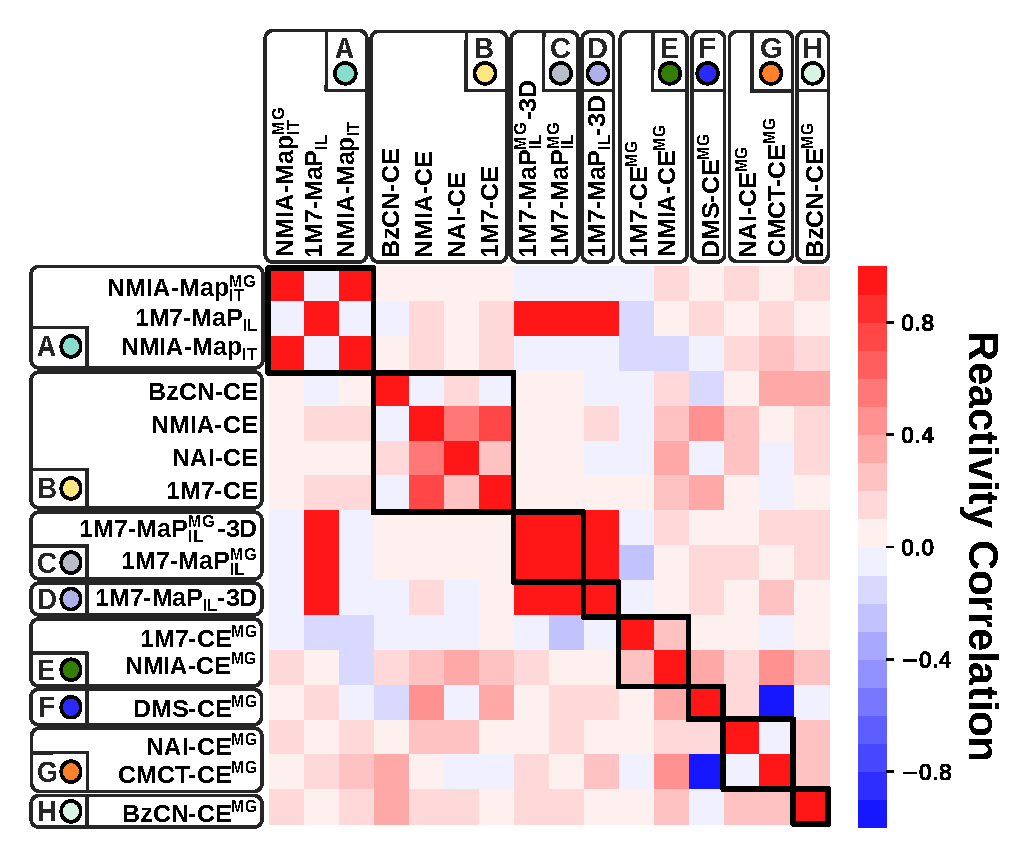
\includegraphics[width=.54\textwidth]{graphs/didy/reactivity_correlation.pdf}\hfill
			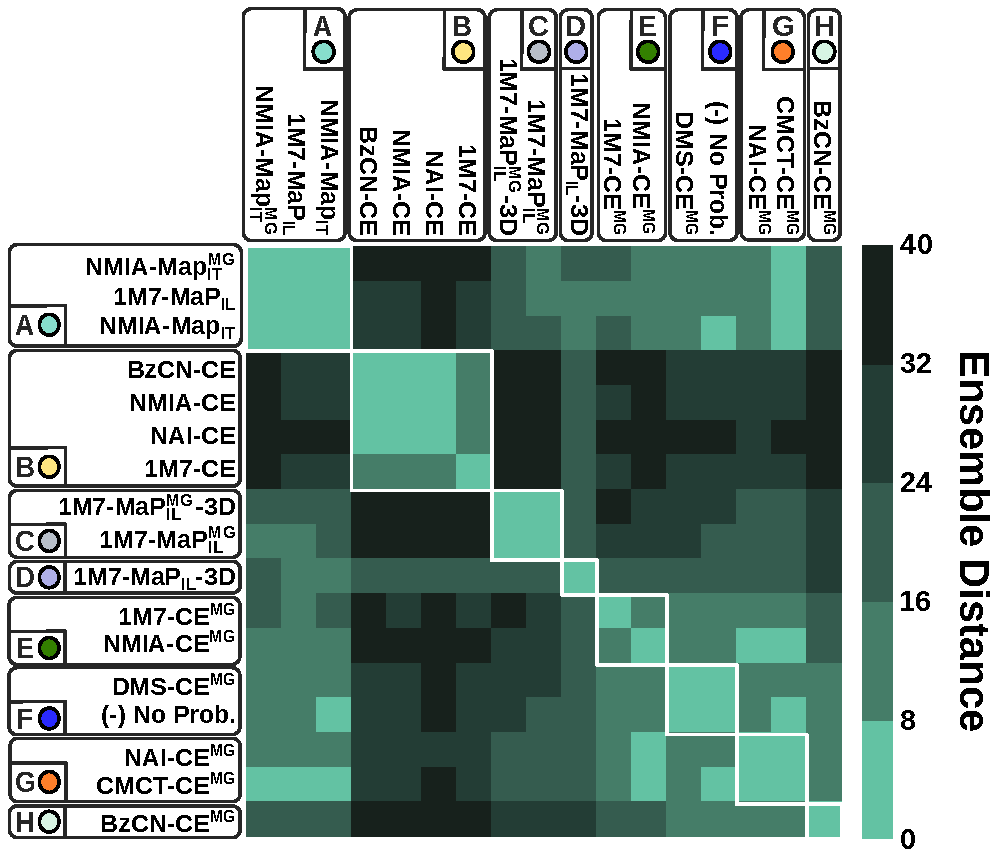
\includegraphics[width=.45\textwidth]{graphs/didy/bi_clustering.pdf}\\
			\noindent Figure~A: Correlation of reactivity profiles (left) and induced (pseudo-)ensemble distance (right). Conditions clustered in our analysis due to their impact of the pseudo-Boltzmann ensemble (black boxes, right) do not necessarily correlate very well in term of raw reactivity (white boxes, left).
			
			
			\paragraph{Correlation metrics and rationale.}To that purpose, we consider the Pearson product-moment \Def{correlation coefficients} $C_{R,R'}$ of two reactivity profile $R$ and $R'$, defined as
			$$ C_{R,R'} = \frac{\sum^n_{i=1}\left(R_i - \mu_R\right)\left(R'_i - \mu_{R'}\right)}{\sqrt{\sum ^n _{i=1}\left(R_i - \mu_{R}\right)^2} \sqrt{\sum ^n _{i=1}\left(R'_i - \mu_{R'}\right)^2}},$$ 
			where $\mu_{R}$ and $\mu_{R'}$  denote the mean reactivity within $R$ and $R'$ respectively. 
			
			The choice of the \Def{correlation coefficient as a measurement of pairwise similarity} for probing profiles is motivated by differences in the distributions of reactivities across experimental conditions and protocols. 
			Indeed, $C_{R,R'}$ remains unchanged by the application of any rescaling, through an affine transformation with positive slope, to either $R$, $R'$ (or both). Moreover, this metrics does not scale with the number of positions.
			Thus, we can restrict the sums and mean values to positions for which reactivities are available in both experiments, and still compare the coefficient with another pair of reactivity profiles. This property is important in order to tolerate \Def{missing values} introduced by experimental artifacts and reagent properties, while still being able to compare the coefficients.			
			
			\paragraph{Results.} We computed the correlation coefficient for all pairs of reactivity profiles, and report the results in the left matrix of Figure~A. For the sake of comparison, we also remind the Ensemble Distance matrix, indicating the difference in impact on the computational predictions of each pair of conditions.
			
			We first observe that almost all of the pairs of reactivity profiles show a positive correlation, as expected from their observation of a common structure. A notable exception is \OneMSevMgCE, having average negative correlation with all its peers (except for \NMIAMgCE). Its outlier status is confirmed by its large ensemble distance to other conditions, yet does not prevent it to achieve a respectable MCC of 70\%. Finally, the perfectly negative correlation between \CMCTMg{} and \DMSMg{} can be dismissed as a computational artifact, since CMCT and DMS react with different nucleotides, and the correlation cannot be computed.
			
			Moreover, we observe that conditions clustered from the Ensemble Distance metrics (due to their impact of the pseudo-Boltzmann ensemble) do not always correlate in term of raw reactivity, with very poor correlations occurring within clustered conditions. This essentially reflects the fact that similar profiles may induce very similar pseudo-Boltzmann ensembles, \emph{ie} different premises sometimes imply the same conclusions. 
			
			Conversely, one observes very few strong correlations outside of clusters. In fact, the only two exceptions are \OneMSevILU and \OneMSevILUThree which, despite belonging to different clusters and achieving different qualities of prediction, correlate almost perfectly with each other and with other reactivity profiles produced using 1M7/SHAPE-MaP. Other natural candidates for explaining the reactivity correlations (Map vs CE, +Mg vs -Mg) do not appear to be supported by this analysis.
			
			Overall, this analysis confirms the consistency of the produced probing profiles (positive correlation), but also suggests a very delicate effect of reactivity data on the downstream predictions, with very different profiles leading to similar predictions (\OneMSevILU), and similar profiles inducing very different ones (\OneMSevILU vs \OneMSevILUThree).}
		
				In particular, while reactivity profiles correlate positively in a pairwise fashion, as can be expected, these results do not support the hypothesis that the method of detection (CE vs Map) would represent a strong differentiator at the level of reactivity profiles. In fact, the only clear clusters are:
		\begin{itemize}
			\item  $\{\NMIAMg,\NMIA\}$;
			\item  $\{\NMIACE,\NAICE,\OneMSevCE\}$;
			\item $\{\OneMSevILU, \OneMSevILUThree,\OneMSevILUThreeMg,\OneMSevILUMg\}$,
		\end{itemize} having respectively a similar reagent, technology, or both, as a common trait. However, neither of those determinants seem universally supported by the observation of the correlation matrix.
		
	}

	\Comment{I am also concerned by the fact that they only have one (-) No Prob condition. For both CE and MaP data, a background subtraction is required. It is not at all clear what the No Prob condition is and why it was not independently subtracted from all the data prior to analysis.}
	
	\Answer{There is a misunderstanding here, the “(-) No Prob” conditions refers to a baseline computational prediction that does not use any probing data as constraints (Turner energy model only). We understand that this may be confusing to the reader, and we now refer to it as “(-) No Exp” for modeling without experimental data.
	
	 Of course we have carried out control experiments without any modification reageant for each of the reported experiments, as now explicitly specified in the material and methods section.}
	
	
	\Comment{I am concerned the MaP data they collected is not reporting on structure. For example, quality controls need to be established showing that DMS reactivities follow expected profiles, i.e. A and C having higher mean reactivity that G and U.}
	
	\Answer{We understand this legitimate concern, expressed by multiple referees. The probing data reported on the structure for each probing conditions and reagents is now provided in Supplementary Figures S3 and S4. Also, please note that the DMS results were not obtained following a SHAPE-MaP-like strategy but by a “classical” RT-stop technique and Capilary electrophoresis.} 
	
	\Comment{The main reason I am concerned with their MaP data is that they used superscript III instead of II for the RT. In the Smola paper, superscript III was attempted, but it was shown it does not detect adduct formation by mutation. If the CE to MaP correlations are low for the data, which I suspect they are, the authors will have to repeat MaP profiling with Superscript II to show this change in the protocol does not affect the data. I suspect however it will and may change the conclusions of the paper.}
	
	\Answer{It is exact that the Weeks laboratory uses an RNAse H minus mutant of the MMLV RT sold as “Superscript II” and advises to use it. However as far as we can tell from reviewing Dr Weeks bibliography, they never reported the test of “superscript III” (another RNAse H- mutant of the MMLV RT sold by the same company), and therefore never showed that this technology does not detect the adduct. 
		
		More precisely, in \cite{Smola2015}, the authors state that “Reaction conditions have been optimized for SuperScript II reverse transcriptase only. Other reverse transcriptase enzymes and derivatives have not been tested and should not be used”. In this work, we tried superscript III in the  described conditions, and inspected the coverage/mutation distribution graphs produced by ShapeMapper. Those graphs are suggested by the Weeks group to assess the success of a SHAPE-MaP experiment, as described in \cite{Smola2015}.
		
	Please find below some examples of the histograms obtained using Superscript III:
	
	\begin{itemize}
	\item \NMIA:
	
	{\centering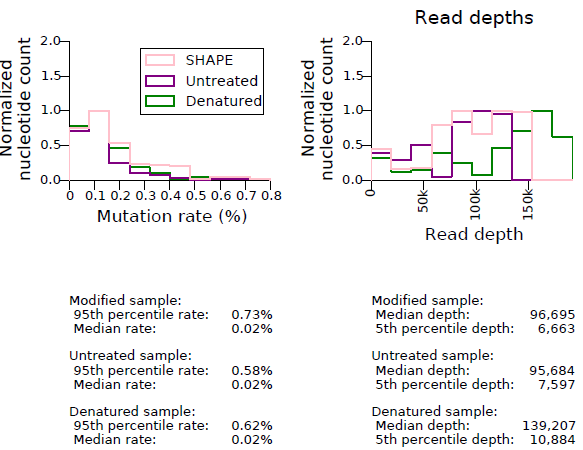
\includegraphics[width=.8\linewidth]{graphs/didy/NMIA}\\}
	
	\item \NMIAMg:

	{\centering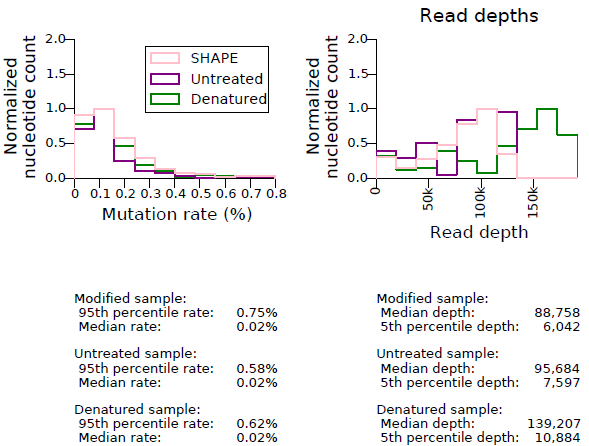
\includegraphics[width=.8\linewidth]{graphs/didy/NMIA-Mg}\\}

	\item \OneMSevILUThree:
	
	{\centering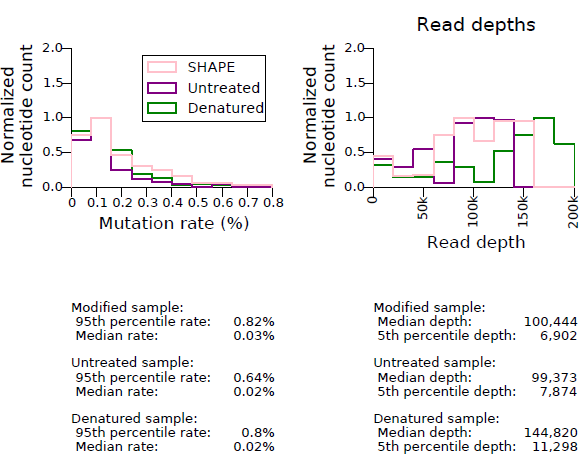
\includegraphics[width=.8\linewidth]{graphs/didy/1M7}\\}

	\end{itemize}
	
	As can be seen on the right  histograms the read depth is sufficient ($>$10k reads/nucleotides) for these experiments to be interpreted (\emph{ie} for the frequency of mutations to be a good estimate of the probability). The histograms on the left shows that there are significantly more mutations in the modified (denatured and SHAPE) samples than in the untreated ones. 
	
	These histograms are very similar to those deemed as exemplary of a successful experiment by \cite{Smola2015},. 
	In addition, those SHAPE-MaP results are consistent with the X-ray structure (see Supplementary Figure S2 and S3), and their use with our prediction software was shown to improve the accuracy of the output model(s). 
	
	In conclusion, a thorough re-inspection of the data does not lead us to question the relevance of these results, and we do not see the necessity to repeat them using superscript II.}
	
	
	\Comment{One possibility if the authors indeed find the MaP data is not correct because of superscript III would be to not include it in the analysis. Unfortunately this may somewhat temper the general interest of the paper, as a majority of SHAPE and probing data is now collected with MaP and -stop protocols.}
	
	\Answer{As discussed above, we did not find any reason to doubt the quality of our results, and believe they should remain included in our analysis.}
	
	\Comment{The authors also need to make their raw data available, I would recommend using the SNRNASM standard (PMID 21610212) and adding the files in the supplement. In addition the raw read files and alignments should really be deposited into the sequence read archive (SRA) so others can assess the quality of the mutation rates.}
	
	\Answer{We agree that raw data should be made available to the reader for the sake of reproducibility. Unfortunately, the SNRNASM resource was no longer available at the time of this revision. We have informed the creators of the resource, but have not witnessed accessibility improvement over the course of our revisions. 
	In the meanwhile, we have deposited the reactivity files on the GitHub page of IPANEMAP, where they also serve as illustrative examples.
	
	We experienced other issues while attempting to upload the raw data onto the SRA. Namely, this database requires a structured definition of the experiment, including several mandatory fields (growth culture...) that we could not reasonably fill given the nature of our experiments. In fact, a cursory search of the database showed that primary data produced by the Weeks lab is very rarely deposited in the SRA, indicating that similar difficulties are also encountered by other groups.
	
	We have permanently uploaded the data at:
	
	{\centering \url{http://www.lix.polytechnique.fr/~ponty/suppdata/ipanemap/}\\}
	
	and commit to its continued accessibility (but will also pursue public venues for better guarantees of a continued availability). 
	}
	\end{enumerate}

\newpage

	\subsection{Reviewer \#2}
	
	\begin{enumerate}[resume]

	\Comment{The authors picked with DiLCrz a hard example since most problems of prediction accuracy are caused by the confusion of the nested structure model in the presence of the reactivities of the pseudoknot. That is, the quite stable PK-subhelix of length 4 (ignored in the nested model and the evaluation) will have a strong impact on reactivities that can not (correctly) be captured. Thus, the authors mainly evaluate how much the prediction of local structures in subsequence 65-120 is correct or not (as also visible in the reported structures within the supplement). Eventually, this also impacts the generality of the results.
	
	Thus, I think the authors should add a respective discussion to the manuscript.}
	
	\Answer{It is true that at least four helices of DiLCrz (DP2, DP2.1, P10 and P9) are somewhat easy to predict, and are indeed consistently found in all predictions, including in the probing-free \Software{RNAfold} MFE prediction. The changes in performances are thus mostly due to the other 6 helices (omitting the pseudoknot). We emphasized this fact in the description of our result section, to provide the reader additional context for the interpretation of our results. However, we disagree that this impacts the generality of our results. In particular, badly produced/poorly combined reactivities may easily disrupt the four above helices, and the fact that our method is able to preserve those helices, yet predict other structure elements, should be considered an asset of our method.
		
	The remark regarding the impact of the pseudoknot subhelix (P7) on the reactivity is very perceptive, and certainly noteworthy. Indeed, positions 111 to 115 (the 5' region of P7) are typically associated with lower reactivities, providing incentives to algorithms for pairing them within their proposed models. Accordingly, one finds those positions to be paired to erroneous partners within most of our models. Such is not the case, however, for the 3' region of P7, which is typically left unpaired in our models.
}
	
	\Comment{The methods section needs some reordering to first formaly introduce clusters and respective measures (stability/support) (e.g. in line 3-1-57) before introducing and discussing MBkM. For this restructuring, you might want to introduce the cummulative sample multi-set "$\mathcal{S} = \sum_d \mathcal{S}_d$" from which the clusters (also multi-sets?!) form a partitioning.}
	
	\Answer{We fully agree that reproducibility is essential, and have realized that our previous manuscript was lacking in details. Accordingly, we have largely revised our description of the method to clarify the nature of the clusters (indeed multisets), and the exact computation of centroids (including base-pair/unpaired position probabilities within a cluster).
		
	However, we have chosen to avoid an overly formal description of the method, as we believe such a writing style would not represent a good fit with the expectations of the typical NAR audience. We have adopted a linear narration of the method, which we completed in the hope to now ensure full reproducibility of the method.}
	
	\Comment{You do not introduce how you are able to compute MEA centroids without explicitely computing base pair probabilities. Checking your source code, I found the bp-probs are computed analogously to the structure probabilities, which is fine but should be explicitely mentioned to be reproducable. 
		
		It is totally unclear to me (and I didnt took the time to track it down in your code), how you derive an MEA for a cluster with structures from different reactivity data sets, since the same structure can be part of the cluster multiple times (with different probe-constraint probabilites). Do you sum up probe-specific probabilities in that case? Do you derive new base-pair probabilities for the cluster (and if so how)?
		
	Please provide somewhere details of your methods concerning the whole bp-prob and MEA centroid computation (at least in the supplementary material). Otherwise, your method description leaves out a central point of your algorithmic pipeline and renders is non-reproducable!}

	\Answer{As mentioned in our response to the previous point, we revised our method description to include more details on the probability distribution on which we base our centroid/MEA structure. The computation of the MEA is performed using a strict reimplementation of the dynamic programming algorithm introduced by \cite{Lu2009}, so we just refer the reader to this article rather than reproducing its content.
		
	Please find below the description of the clustering method, as now appears in our revised document.
		\Quote{\paragraph{Clustering across conditions.} In order to infer recurrent conformations across sampled sets, \OurTool{} agglomerate structure (multi)sets while keeping track of their condition of origin, and \Def{clusters} with respect to the \Def{base-pair distance}, the number of base pairs differing between two structures. A clustering algorithm then partitions the (multi)set of sampled structures into \emph{clusters}, (multi)sets of structures such that the accumulated sum of distances over clusters is minimized.
				
				Among the many available options, we chose the Mini Batch k-Means algorithm~\citep{Sculley2010} (MBkM), implemented in the \Software{scikit-learn} pacakage~\cite{Pedregosa2012}, which requires less computational resources than the classic k-means algorithm, yet performed similarly in preliminary studies as an extensive collection of both agglomerative (affinity propagation) and hierarchical (Ward, Diana, McQuitty) clustering algorithms. A dissimilarity matrix, presenting the pairwise base-pair distance between structures, is precomputed and fed to the clustering algorithm.
				
				Any cluster $C$ output by the clustering is a multiset of structures, each labeled with its origin condition of $\mathcal{D}$.
				The \Def{cluster probability of a structure feature} $f$ (base pair or unpaired base) within a cluster $C$ is then defined as 
				$$ \mathbb{P}_C(f) = \frac{\sum_{\substack{S\in \mathcal{C}\\\text{s.t. } f\in S}} e^{-E(S)/RT}}{\sum_{\substack{S'\in \mathcal{C}}} e^{-E(S')/RT}} $$ 
				where $R$ represents the Boltzmann constant, $E(S)$ is the Turner free-energy, and $\mathcal{C}$ is the (non-redundant) set of structures in $C$. From those probabilities we define the \Def{centroid structure} of a cluster as its Maximum Expected Accuracy (MEA) structure, computed efficiently following Lu\etal~\citep{Lu2009}.
				
				Moreover, define the (pseudo-)\Def{Boltzmann condition probability} of a structure $S$, generated for a probing condition $d$ as part of a sampled  set $\mathcal{S}_d$, as
				$$\mathbb{P}_d(S) = \frac{e^{-E_d(S)/RT}}{\mathcal{Z}^*_d} \text{, with } \mathcal{Z}^*_d := \sum_{S'\in \mathcal{S}_d} e^{-E_d(S')/RT}$$
				where $E_d(S)$ is the pseudo free-energy assigned to the structure $S$ within the probing condition $d$.
				The \Def{stability} of a cluster $C$ denoted its accumulated pseudo-Boltzmann probability across conditions, computed as
				$$\text{Stability}(C) = \sum_{d\in \mathcal{D}} \sum_{S\in C\cap \mathcal{S}_d}  \mathbb{P}_d(S).$$
				A cluster is deemed \Def{significantly populated} if its stability exceeds a predefined threshold $\epsilon$. 
				We set  $\epsilon =\#{\sf Datasets}/3$ by default, such that at most three clusters are deemed significantly populated, and used as our primary candidates.
				Finally, we consider two clusters to be \Def{highly similar} if their centroid structures differ by at most $\delta$ base pairs ($\delta=1$ by default), allowing the identification of clusters in the presence of minor variations.
				
				
				
				
				The targeted number of clusters is a critical parameter of the \CL{} algorithm. It should, at the same time, remain small enough to ensure reproducibility, while being sufficiently large to discriminate outliers and ensure consistency within each cluster. We determine an \Def{optimal number of clusters} $\NumClust$ using an iterative heuristics, gradually increasing the number of clusters until a significantly-populated cluster is split into two similar clusters, or a poorly populated (outlier) cluster is created.
				Namely, our iterative heuristic consists in running \CL over an increasing number $\NumClust$ of clusters, starting with $\NumClust=2$, until the following \Def{stopping criterion} is met: 1) Two significantly populated clusters have associated centroids which are highly similar; or 2) Centroid structures of significantly populated clusters from the previous iteration are highly similar to those of the current iteration.}
}
	
	\Comment{Please replace "kT" by "\text{R}T" in the structure probability formula (and wherever needed)!}
	
	\Answer{We agree that using $k$ was unfortunate in this context, leading to an unnecessarily notational overload, and have used $R$ instead as suggested.}
	
	\Comment{What is the difference betwee the "cummulative probability of [a cluster's] structures" (line 3-1-58) and the formally introduced "Stability(C)" notion? If there is none, please use accordingly, otherwise provide respective details.}
	
	\Answer{Those two notions indeed coincide and we had initially used a sentence to avoid a forward definition. We have now moved the stability definition earlier in the method description, and use it to define the notion of \Def{significantly populated cluster}.}

	\Comment{Please provide (eg in the supplement) some further details how to derived the values for m abd b for the Deigan method. So far, the description is quite vague. Within this context, you might want to discuss that too low pseudo-energy boni will yield similar results as hard constraints (which you want to avoid).}
	
	\Answer{The values $m$ and $b$ were loosely calibrated by grid search based on the \cite{Cordero2012} dataset, revealing a limited influence of those factors on the predictive performances. }

	\Comment{The formula for "$Stability(C)$" misses a "$\sum_{S\in C \cap \mathcal{S}_d}$" between the sum over d and the probability.}
	
	\Answer{Absolutely, this is now fixed.}

	\Comment{Please put brackets around the probability sum within the "$Support(C)$" definition to make clear that you are comparing $\tau$ to the sum.}
	
	\Answer{Thanks for the suggestion, which greatly improves the readability of the formula.}

	\Comment{If I get it right, if you are facing two clusters, one dominant in stability and the other in support, you will report two centroids, right?
	So reactivities that are inducing very high stability might dominate your prediction? Please check this hypothesis and if true discuss within the manuscript!}

	\Answer{
		The interpretation of the reviewer is accurate, and it is true that the configuration of reactivities may give rise to \Def{tight} (focused on a few structures), or \Def{wide} (compatible will multiple conformers) pseudo Boltzmann Ensembles. Combining a \emph{tight} and \emph{wide} pseudo-Boltzmann ensembles will grant more influence to the former over the final prediction. 
		In the worst case scenario, the combination of a poorly-informed tight Ensemble, which we informally call a \emph{bully}, with an accurate wide (\emph{open-minded}) Ensemble, may lead the bully to almost solely drive the ultimate prediction. However, we believe such cases to be rare, as indicated by the good performances of our approach on single probing experiments and that, in general, tight ensembles are indicative of successful experiments.
		
		Moreover, in the presence of multiple probing conditions, bullies can be overruled by a population of informed, even if open-minded, individuals. Our approach can indeed be seen, in first order approximation, as a weighted voting mechanism where each voter splits his vote between her/his preferred candidates. Since the probability of independently ill-informed bullies to agree by chance decreases exponentially with their number\footnote{In the absence of a systematic underlying bias, synchronizing the bullies, which in itself would be informative, or at the very least worthy of investigation.}, the voting process will ultimately favor a population of open-minded individuals over a, possibly majority, subpopulation of bullies. 
		
		Finally, it is worth reminding that reactivity values are normalized, so that the average reactivity (over nucleotides touched by the probe) remains the same across conditions, so that the probability of a tight Ensemble being an artifact due to a given probing condition is expected to be limited. 
	}
	
	\Comment{If you are NOT reporting multiple structures (as indicated in your results) how do you deal with cases illustrated above?}
	
	\Answer{
		Over a normal execution, \OurTool{} {\bf does report} all the dominant clusters (and even dominated ones), along with their centroids.
		In the context of benchmarking, unless explicitly specified, we systematically picked a cluster uniformly at random from the output to assess the predictive performances. 
		
		However, in an overwhelming proportion of our experiments, a single cluster is reported, due to a generally good correlation  of stability with support. For instance, it is mathematically impossible for a single condition to feature more than one Pareto cluster, since the cluster $C^\star$ having max stability $s^\star$ is such that: either $C$ has support $t^\star=1$, in which case it dominates any other cluster with signature $(s<s^\star,t\in\{0,1\})$; or $C$ has support $t^\star=0$, ruling out the possibility of $t=1$ for any other cluster (since it would imply $s>s^\star$). 
		
}
	
	\Comment{On page 7 you write "Fig. 5 suggests the presence of 8 clusters", which I do not agree... for me the PCA depiction would yield 4 clusters, i.e. B, C, D and the merge of all others. Thus, please rephrase the sentence or provide some other reason why you came up with 8 clusters from the beginning..}
	
	\Answer{We respectfully disagree, and still see 8 clusters in the PCA (and distance matrix, which we reformatted and reproduced below). Of course, this view is quite subjective and we carefully chose our wording (\emph{suggest}) to reflect the inherent limitations of a visual inspection. 
	\Quote{
			{\centering 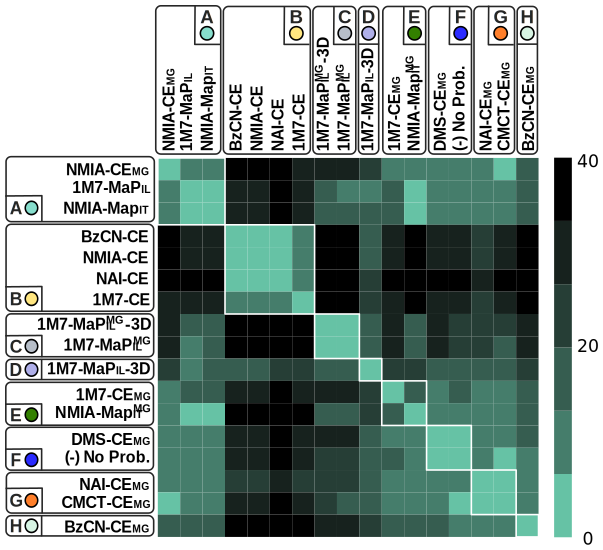
\includegraphics[width=.75\linewidth]{graphs/didy/bi_clustering}\\}%
		}
	On a more objective level, an examination of the distance matrix above indicates that merging conditions in the clusters A, E, F, G and H as suggested would be ill-advised, since some of the pairs of clusters ((E,F,G) vs H, A vs E\ldots) are actually quite distant. This  fact is somewhat obfuscated by the low-dimensionality of the PCA.
}
	
	\Comment{Concerning data normalization (Cordero et al.): when resetting all non-reacting position to 0, dont you loose the "background noise" of the experiment? 
	Did you test other options like subtracting the minimum/average/maximum of all non-reacting positions from all reactivities (before setting non-reacting to zero)?}

	\Answer{
		First, we need to stress that this cancellation of non-reactive nucleotides only applies to DMS and CMCT probing, and reflects the fact that those reagents are not supposed to react with certain nucleotides. Namely, DMS only reacts with \Ab{} and \Cb{}, while CMCT only reacts with \Gb{} and \Ub{}. We did verify that the reactivities associated with non-reacting nucleotides, as assessed using the relevant formula, are overwhelmingly close to zero so normalizing by the minimum/average/maximum would have no effect. Overall, these observations strongly support the idea of non-informative reactivity values at those positions. For instance, using them within the computation of the normalization (based on a percentile) would systematically increase the average reactivity, leading the pseudo-energy bonuses to act as \emph{hard constraints} for all practical purposes.
		
		Moreover, the reactivity normalization is based on percentiles over reacting positions, and there is no reason to suspect a systematic bias between the nature of nucleotides and the structural context. It follows that the effect of the normalization should be very similar when starting from a fully informed reactivity profile, or ignoring reactivities associated with \Gb{}/\Ub{} nucleotides.

		Finally, we must point out that we do not set the reactivities of non-reacting nucleotides to $0$, but rather to \emph{non-reactive}, usually encoded as a large negative value. This value is then interpreted as a missing data within \Software{RNAfold}, so that no pseudo-energy (rather than the bonus induced by a reactivity of $0$ by the \cite{Deigan2009} conversion) is used for those positions.
		
		

}
	
	\Comment{I would be very interested to see the performance of multi-probe predictions via RNAfold (MFE+MEA) when merging their reactivity data.
	For instance: just average the reactivities (per position) and provide them as new pseudo-reactivity data to RNAfold.
	While this might extremely mess up predictions, it might also yield similar effects as IPANEMAP, i.e. importance of contradicting reactivities is reduced the more experiments are considered..}
	
	\Answer{
		In principle, this idea of averaging reactivities is natural, but has limits. 
		In particular, it does not sample from the same distribution as our approach, as can be seen in the following toy example:
		
		{\centering
			\begin{tabular}{ll}
				Structure $S^\star$ (free-energy $E^\star$)& \texttt{(((..)))(((..)))} \\
				Structure $S^\varnothing$ ($E^\varnothing=0$)& \texttt{................} \\
				Reactivity profile $r^\alpha$                          & \texttt{0011100000000000} \\
				Reactivity profile $r^\beta$                          & \texttt{0000000000011100}
			\end{tabular}\\}
		
		Now, consider a simplified ensemble of structures, consisting only of $S^\star$ and $S^\varnothing$, the open chain having free-energy $E^\varnothing = 0$. 
		Given a structure $S$ and a reactivity profile $r$, the overall pseudo-energy bonus is then 
		$$ \Delta G_r(S) = \sum_i m \log(r_i+1) + b.$$
		The energy bonuses for the combinations of structure/(averaged)reactivity profiles are 
		
			$$
			\begin{array}{c|cc}
				\Delta G_r(S) & S:=S^\star & S:=S^\varnothing\\ \hline
				r:=r^\alpha & 2m\log 2 + 4\, b & 3m\log 2 + 16\, b\\
				r:=r^\beta & 2m\log 2 + 4\, b & 3m\log 2 + 16\, b\\
				r:=\frac{r^\alpha+r^\beta}{2} & 4m\log 3/2 + 6\, b & 6m\log 3/2 + 16\, b			
				\end{array}
			$$
		
		
		For instance, the emission probability of $S^\star$ given a reactivity profile $r$ is
		\begin{align*}\mathbb{P}(S^\star\mid r) &= \frac{\displaystyle e^{-\frac{\Delta G_{r}(S^\star) + E^{\star}}{RT}}}{\displaystyle e^{-\frac{\Delta G_{r}(S^\star) + E^{\star}}{RT}} + e^{-\frac{\Delta G_{r}(S^\varnothing)}{RT}} }\\
		&= \frac{1}{1 + e^{\frac{\Psi(R) + E^{\star}}{RT}}}
		\end{align*}
		with  $\Psi(r) := \Delta G_{r}(S^\star) -\Delta G_{r}(S^\varnothing)$.
		
		It follows that the expected frequency of occurrences of $S^\star$ within an overall multiset of $M$ structures sampled by \OurTool{} ($M/2$ structures for each condition) is given by 
		\begin{align*}
		\mathbb{E}\left(\frac{\#\text{Occ}(S^\star)}{M}\mid r^\alpha \wedge r^\beta\right) &= \frac{\mathbb{P}(S^\star\mid r^\alpha) + \mathbb{P}(S^\star\mid r^\beta)}{2}\\
		 &= \frac{1}{1 + e^{\frac{-m \log(2) -12\,b + E^{\star}}{RT}}} \\
		 &= \frac{1}{1 + \frac{e^{\frac{-12\,b + E^{\star}}{RT}}}{2^m}}
		\end{align*}
		while the same quantity, measured within $M$ structures sampled from an averaged reactivity profile $\frac{r^\alpha+r^\beta}{2}$, becomes
		\begin{align*}
			\mathbb{E}\left(\frac{\#\text{Occ}(S^\star)}{M}\mid \frac{r^\alpha+r^\beta}{2}\right) &= \frac{1}{1 + e^{\frac{\Psi\left(\frac{r^\alpha+r^\beta}{2}\right) + E^{\star}}{RT}}}\\
			  &=\frac{1}{1 + \frac{e^{\frac{-12\,b + E^{\star}}{RT}}}{(3/2)^{2m}}}.
		\end{align*}
		The two quantities are strictly different for any value of $m$ (except $m=0$), and the ratio of probability can go in different directions depending on the reactivities profiles and (exponentially large) ensembles of conformations.
		
		More empirically, we believe such a strategy would impact the robustness and versatility of our whole approach. 
		Indeed, in the presence of two sources of reactivities showing strong disagreement, indicating either the probing of two conformations, or an erroneous condition, averaged reactivity terms will end up favoring unpaired conformations, while our approach will probably produce two clusters (leaving aside the final Pareto optimization).
	}
	
	
	\Comment{Given your tool's documentation, a couple of questions arise that should be answered within the README.
		
	\begin{itemize}\item How are the reported free energies evaluated since your predictions are based on (multiple) reactivity-biased predictions? (your code hints at RNAeval calls, but please be verbose in the documentation to enable a clear intepretation of the results and comparability with other tools' output)\end{itemize}}
	
	\Answer{Free-energies are re-computed using the \Software{RNAeval} tool, we have completed the documentation to make this point more explicit (and refer to a refined definition of these terms in the manuscript).}
	
	\Comment{\begin{itemize}\item How are the reported Boltzmann probabilities computed? based on the overall sample set? the respective cluster? (in both cases: what energies are used?) or based on the true (unconstraint) partition function computed e.g. by RNAfold?\end{itemize}}
	
	\Answer{The reported Boltzmann probabilities, also called Stability in the manuscript, are strictly computed as described in the manuscript. We have made this point explicit in our revised documentation.}
	
	
	\Comment{Given Table 1 (CMCT) and the general unawareness of the Nussinov-like MEA-optimization of the importance of base pair stacking, you might be able to further improve your results when implementing an MEA variant that excludes lonely base pairs.}
	
	
	\Answer{We agree that this would be a potentially fruitful development. This would require a modification of the dynamic programming equations presented by \cite{Lu2009}, for instance by leveraging the Waterman grammar into something similar to:
	\begin{align*}
	  S &\to \texttt{(}\texttt{(} \,T\, \texttt{)}\texttt{)}\, S \mid \texttt{.}\, S \mid \varepsilon \\
	  T &\to \texttt{(}\, T\, \texttt{)} \mid \texttt{(}\texttt{(} \,T\, \texttt{)}\texttt{)}\, U\mid   \texttt{.}\, S \\
	  U &\to \texttt{(}\texttt{(} \,T\, \texttt{)}\texttt{)}\, S \mid \texttt{.}\, S 
	\end{align*}
	Such a modification would triple the memory requirement, but would remain polynomial in time and should not constitute the bottleneck of the whole method. However, it would also warrant an extensive validation effort, and lead to the description of further material within an, already consequent, Methods section. For these reasons, we prefer to leave this promising extension to a future version of \OurTool.}
	
	\Comment{I highly recommend to integrate IPANEMAP into the package management system conda via the bioconda channel. This would:
		\begin{itemize}
	\item be easy since IPANEMAP is eventually a set of python scripts (only a simple build and dependency script needs to be integrated into bioconda's recipes github repo)
	\item  handle all dependencies for the user
	\item ensure a simple installation of the tool and all dependencies 
	\item increase visibility of the tool
			\end{itemize}}
		
	
	\Answer{Again, we agree that integrating the package within \Software{conda} would be ideal. However, since the \Software{ViennaRNA} package is not currently available on \Software{bioconda} for all platforms (only Mac OS and Linux), this would still require a manual installation and would somewhat mitigate the benefits of such an integration. 
		
		In the new version of the documentation, we at least partially ease the installation process, and suggest using \Software{pip} (available in any \Software{Python} release) to install all the necessary dependencies through the command:
		
		{\centering \Software{pip install cython scipy numpy sklearn}\\[.5em]}
		
		The \Software{ViennaRNA} package, however,  still needs to be independently installed. We have contacted the maintainers of the \Software{ViennaRNA} package to (help) make the package more universaly accessible, and will certainly pursue the  integration of future versions of \OurTool{} within \Software{bioconda} (a port to \Software{Python3} is currently underway).
	}
	
	\Comment{When reading your work, it reminds me of another application, ie. the computation of unpaired probabilities for RNA-RNA interaction prediction in the presence of multiple probing data. For instance, see 
	https://doi.org/10.1093/bioinformatics/bty1029
	where single-experiment-reactivities were integrated (via Vienna package routines). 
	Given your pipeline, you should be able to derive suitable probabilities either directly from Pareto-optimal cluster(s) or from the overall sample set.}
	
	
	\Answer{This is a great suggestion for a future application of our method, and will rank high within the list of our priorities (along with the, arguably natural analysis of multi-states RNAs). However, we feel that such a study would warrant a validation effort that would go beyond the scope of the current paper.}
	
	\Comment{Fix the following typos/unfortunate choices of words:\begin{itemize}
	\item general: et al $\to$ et al. \IAnswer{Done}
	\item 1-2-30 : please provide the abbreviation details for SHAPE \IAnswer{Done}
	\item 1-1-21 : remove comma after "experiments" \IAnswer{Done}
	\item 1-2-37 : "more dynamics"\IAnswer{Done}
	\item 1-2-49 : "qualitative"\IAnswer{Done}
	\item 1-2-53 : "of individual nucleotides"\IAnswer{Done}
	\item 2-1-23 : "These include " beside structure optimization " the joint folding.."\IAnswer{Done}
	\item 2-1-49 : signal $\to$ signals\IAnswer{Done}
	\item 2-2-38 : criterion "are" $\to$ "is"\IAnswer{Done}
	\item 2-2-39 : identified $\to$ represented\IAnswer{Done}
	\item 3-1-5 and 8 : better replace "$R_i$" with "$d_i$", since you are using R for reference later on \PAnswer{We replaced $R_i$ with $r_i$ to avoid clashing with the new notation for the Boltzmann constant $R$. We also denote the reference structure as $\Ref$ in the definitions of the evaluation metrics.}
	\item 3-1-60 : maybe replace "\#Datasets" with "$|\mathcal{D}|$" ? \IAnswer{Done}
	\item 3-2-17 : missing "are" in "that both" \IAnswer{Done}
	\item 3-2-32 : move "where $k$ is the number of clusters" to line 40, where it is needed. \IAnswer{Done}
	\item 4-1-8 : Within the formula "$Dist(d,d')$" you have to replace "$x$" with "$i$" \IAnswer{Done}
	\item 4-1-52 : "Non-canonical" $\to$ "Crossing" or "Pseudoknot-forming" \PAnswer{We clarified this description, which originally mixed the notions of non-canonical BPs and pseudoknots in a confusing manner. The new sentence reads \Quote{Non-canonical base pairs were removed, and a non-pseudoknotted secondary structure was extracted as a maximum subset of non-crossing base pairs~\citep{Smit2008}.}}
	\item 5-1-40 : "metrics" $\to$ "metric" \IAnswer{Done}
	\item 6-2-44 : "hajdin" $\to$ "Hajdin" \IAnswer{Done}
	\item 8-1-31 : "Figure 1" $\to$ "6" \IAnswer{Done}
	\item 10-1-56 : "Figure" $\to$ "Table" \IAnswer{Done}
		\end{itemize}}	
	\end{enumerate}
	
	\newpage
	\subsection{Reviewer \#3}
	

	\begin{enumerate}[resume]
	\Comment{My primary concern is that the authors use a pseudo-free energy formulation (page 3) with parameters that are the same for all conditions and probing reagents.  I am very surprised that this works.  The \cite{Deigan2009} work fit the parameters empirically for SHAPE data.  \cite{Eddy2014} more explicitly drew the connection between these parameters and the log odds ratio of a nucleotide being paired, following earlier work of \cite{Suekoesd2013}.  \cite{Cordero2012} also explicitly fit the log odds for DMS data using gamma distributions.  I would expect that each probing reagent and each probing condition would need different parameters.\label{arg:homogenous}}
	
		\Answer{We also expect that additional conversion formulae, and a specific parameter calibration, for each condition, would be beneficial to the downstream predictive performances. In fact, it is one of our ongoing (recently funded) projects  to produce more extensive data for a subset of the conditions explored in this study, and to attempt to systematically learn reactivities-to-pseudo-energy conversion models. 
			
		However, the conjunction of:
		\begin{itemize}
			\item Distinguishable, yet large-variance and highly-overlapping, reactivity distributions being observed for unpaired and paired nucleotides;
			\item High reproducibility for  reactivity profiles across repeats (and, albeit less frequently, across probes as shown in Figure A above);
		\end{itemize}
		supports the notion that the determinants of SHAPE reactivity extends far the current binary paired/unpaired model. 
		This hypothesis is already explored to some extent in \cite{Suekoesd2013}, and confirmed by recent mechanistic studies~\citep{McGinnis2012,Sexton2017,Hurst2018,Mlynsky2018,Frezza2019,Busan2019}. 
		
		This leads us to a strong suspicion that future pseudo-energy models will have to consider more structural contexts than the current binary one. Those contexts will need to be captured by the dynamic programming schemes. The training of such extended models would probably induce a highly heterogeneous quality for pseudo-energies models trained across conditions, given  the relative scarcity of available data for certain reagents/technologies. In particular, training extended parameters would probably lead to overfitting in contexts where only a couple of reactivity profiles are currently available.
		
		
		Moreover, going back to the suggested use of the gamma distribution in the case of DMS, it is worth pointing out that \cite{Cordero2012} state in their supplementary material that
		\Quote{
		The performance of the algorithm using this probabilistic potential for SHAPE, DMS, and CMCT reactivities is given in Table S6 and is identical to
		results obtained for the standard potential with slope $m$ and intercept $b$ optimized through grid
		search .}
		We also note the relative stagnation of performances of state-of-the-art tools integrating SHAPE data, despite an increasing sophistication of the pseudo-free-energy models. So, while we believe progress can be made in the integration of reactivities, we do not expect them to radically change the quality of predicted models, nor to invalidate the findings described in this manuscript.
		
		To summarize, it seems too early in this manuscript to pursue a specialization of energy models to each reagent/probing technology, and the benefits of considering comparable reactivity profiles (produced in an homogeneous manner, and similarly normalized) far outweigh the expected loss in predicting accuracy. Consequently, rather than specialize our treatment of individual probes and address this heterogeneity as a possible confounding factor in our analyses (in a way that would remain to be determined), we prefer to preserve a homogeneous treatment for all sources of probing data. 

		}
	
	\Comment{The manuscript needs to be clearer about how the two parameters (m and b) determined for this work.  What optimizations were performed?  It needs to be clear that proper cross-validations were performed if the parameters were optimized.  Conversely, if the optimizations were not performed, it seems like an opportunity was then lost to have the best accuracy.}
	
		\Answer{
			The (hyper)parameters $m$ and $b$ were initially calibrated on the \cite{Cordero2012} dataset, revealing a very limited impact of the parameters on the prediction accuracy. We kept those values for multi probing, as the scarcity of available data did not allow us to afford an extensive cross-validation. We updated the description as shown below to be more explicit.
			\Quote{
			Those values were halved in comparison to those recommended by Deigan\etal\citep{Deigan2009}, following both a grid search optimization on the Cordero dataset, and based on the rationale that lower absolute values for pseudo-energy bonuses increase the expected overlap between pseudo-Boltzmann ensembles.}
		}
	
	\Comment{I am also concerned that the manuscript is not as clear as it should be about the three types of multiple data that are used.  It can use multiple reagents, probing data for multiple solution conditions, or probing data across multiple sequence variants (a.k.a. mutate and map data).  It is a real achievement that one program handles all three cases.  The abstract does state this (briefly).  The Introduction is not clear on this points, just calling the data “multiple probing data.”  Also, the text itself is sometimes unclear about what is meant.  On page 6, for example, the sentence “It is also worth mentioning that NMIA+CMCT, combining the best and worst conditions, achieves a better combined performance than DMS+NMIA, the two best mono-probing conditions.” calls these “multiple conditions”, but these data are from multiple probing reagents.  I would like to see a revised manuscript be clearer about the three types of information in the Introduction.  In the text, multiple reagents, multiple solution conditions, and multiple sequence variants should be clearly denoted as different multiple data types. }
	
	\Answer{
	  In the revision, we clarified several times, including at the very beginning of the Methods section, that the term "condition" encompasses a wide variety of contexts (reagent, probing technology, ionic concentrations, and sometimes even structurally-homologous mutants) leading to the production of a reactivity profile. 
	}
	
	\Comment{My third concern is that IPANEMAP is not entirely stable, in that there are variations in the results from run to run.  Users of the software will want the overall results to be stable; it is hard for most users to use a program multiple times and integrate the results.  It seems to me that the stability would be improved by using larger sample sizes, and that this should be explored for this manuscript.  If larger sample sizes don’t improve the stability, this should be addressed. }
	
	\Answer{
		We agree that stability of the predictions is potentially problematic, especially in the context of reproducing earlier results. 
		
		Larger sample sizes represent a natural option for stabilizing the predictions, and indeed seem to decrease the variability. However, a substantial increase of the number $x$ of samples induces extreme computational demands, due to the current necessity to compute the dissimilarity matrix in $\Theta(x^2.n)$ time and $\Theta(x^2)$ memory. In this context, simply multiplying by 10 the number of samples would induce a 100 fold increase of the time requirement. In the future, we will revisit the clustering component to learn suitable embeddings for secondary structures, granting access to linear-time EM algorithms (eg based on Gaussian Mixture Models).
		
		\Quote{
	{\centering 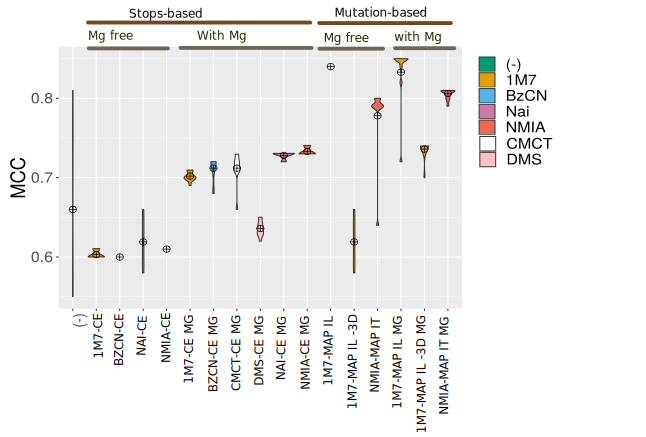
\includegraphics[width=.7\linewidth]{graphs/boxplotreproducibility}\\}
}					
		Moreover, as noted by this reviewer, an expert user would ensure a greater stability by running \OurTool several times (say 10), and electing the most recurrent structure. This process would achieve asymptotic determinism, since the frequency of a structure would converge towards real emission probabilities. Moreover, most frequent structures seem to be the best quality ones, and are emitted by \OurTool with fairly large probability, ensuring convergence in a reasonable number of iterations.
		However, such a process would be cumbersome for a basic user.
		
		In the future, for the sake of reproducibility, we also wish to report, and letting the user specify, a \Def{random seed}, which will  allow the exact reproduction of an analysis. However, random seeds are currently not supported by \Software{RNAsubopt}, so we are working towards their inclusion within the \Software{ViennaRNA} package.
	
	}
	
	\Comment{On page 3, the text states that “Non-canonical base pairs were removed (40), by considering as the secondary structure the maximum subset of non-pseudoknotted base pairs.” I think the manuscript should state that non-canonical pairs were removed and that pseudoknots were also removed.  Just removing the pseudoknots would not remove the non-canonical pairs. }
	
	\Answer{This is entirely correct. We clarified this description, which originally mixed the notions of non-canonical BPs and pseudoknots in a confusing manner. The sentence now reads: \Quote{Non-canonical base pairs were removed, and a non-pseudoknotted secondary structure was extracted as a maximum subset of non-crossing base pairs~\citep{Smit2008}.}}

	\Comment{On page 5, the MCC should be stated as the compromise between sensitivity and PPV (not sensitivity and specificity).}
	
	\Answer{While the statement was meant to be informal, we agree (and it is quite established in the field) that the sensitivity is not a relevant metric for assessing the predictive capacities of structure prediction methods, and that the MCC correlates very well with the product of the Sensitivity and PPV. We have decided to preserve the informal tone, and now state: \Quote{It can be interpreted as a compromise between the main metrics derived from the confusion matrix, and is defined as [..] }}

	\Comment{Figure 2 shows the accuracy of structure prediction using NMIA, DMS, and/or CMCT data.  As noted above, the pseudo free energy parameters for SHAPE (NMIA) will not be optimal for DMS and CMCT.  The benchmarks should therefore also be run using the pseudo free energies fit by the Das lab for DMS and CMCT~\citep{Cordero2012}.  My hypothesis is that the structure prediction accuracy will be higher with the properly fit parameters.}
	
	\Answer{
		Unfortunately, due to our current reliance on \Software{RNAfold}, which takes reactivities as input rather than direct pseudo-energy terms, we could not test this hypothesis. However, we do not expect such a fitting procedure to produce substantially better results. Indeed, as stated in the supplementary material of the \cite{Cordero2012} manuscript:
		\Quote{The performance of the algorithm using this probabilistic potential for SHAPE, DMS, and CMCT reactivities is given in Table S6 and is identical to results obtained for the standard potential with slope (m) and intercept (b) optimized through grid-search.}
		While this leaves open the possibility of improvements upon re-optimization of the $m$ and $b$ parameters, this statement indicates that the nature of the conversion itself does not play a large role in the final performances. 
	}

	\Comment{In the Conclusion and Discussion, it is an oversimplification to state that Rsample also uses stochastic sampling.  Rsample attempts to adaptively define the pseudo free energies to not perturb probabilities for nucleotides in an initial stochastic sample that are consistent with the SHAPE mapping data.  Perhaps this manuscript should also mention that detail and state this adaptive approach is possibly not as accurate (when producing a single structure) as the \cite{Deigan2009} approach.}
	
	
	\Answer{
	This refined free-energies could indeed be impacting the predictive capabilities of \Software{RSample} (although their underlying rationale is convincing), we came to realize upon further inspection that \Software{RSample} actually never uses sampling/clustering on the \cite{Hajdin2013} dataset. Rather, the method concludes from the corrective factors that a single conformation is most likely, and simply returns the MEA of the whole pseudo-ensemble. We have updated our discussion to include this alternative explanation, which seems to explain the strong discrepancy, and supports the notion that clustering can be used to \emph{clean up} a noisy Boltzmann ensemble.
	\Quote{
In this context, the good performance of \OurTool in comparison with \Software{RSample}~\citep{Spasic2017} may appear surprising. Indeed, while independently developed and used~\citep{Deforges2017}, both methods share a common sampling/clustering scheme. However, \Software{RSample}~\citep{Spasic2017} reverts to a MEA~\citep{Lu2009} computation whenever a single conformation is suspected. The MEA structure coincides with the centroid of the whole Boltzmann ensemble, suggesting that the increased performances of \OurTool could be at least partially attributed to the use of sampling, and to our adaptive choice of the number of clusters.
Moreover, even in cases where a single dominant conformation is expected, considering multiple clusters seems to create more opportunities for discarding noisy random unstable conformations. Such conformations naturally occur in a Boltzmann-distributed subset of structures, and may end up \emph{polluting} the centroid structures by artificially inflating the cluster diversity. }}

	\Comment{Typos, etc.:
		\begin{itemize}
		\item The quality of writing is excellent.  There are few typos and the text is clear.  
		\item I noted in the second column on page 3 that k is defined before the equation that uses it (1/(1+k)).  It would be more conventional to define k after the equation.  (I thought I had missed something as I read through).  \IAnswer{Done}
		\item In the Funding section, “phD” should be “PhD”. \IAnswer{Done}
		\item There are many problems with the references, however.  Many references are incomplete (missing page and volume, e.g. 22, 23, …).  A number of references also have superfluous months with the years (e.g. 5, 6, 7,…). \PAnswer{We have extensively sanitized our references, and we believe our bibliography now adheres to accepted standards.}
		\item It would be helpful if the caption to figure 2 named the benchmark dataset.  This is clear in the main text, but will make it easier to quickly digest the manuscript if the captions are all self-contained.\PAnswer{We have systematically revised the captions to make the as self-contained as possible, and in particular always name the dataset on which the data was produced.}
	\end{itemize}
}
	

	
	\end{enumerate}
\newpage
	
	\subsection{Reviewer \#4}
	
	\begin{enumerate}[resume]


	\Comment{IPANEMAP is benchmarked against Rsample in a mono-probe setting. It is shown to outperform Rsample, where the authors attribute this to the sample denoising IPANEMAP performs via clustering (page 7). I am not sure if this is indeed the case and also think this benchmark could be improved in several ways.}

	\Answer{First of all, we would like to point out that the performances of \OurTool{} in a mono-probing setting were explored as a validation of the basic predictive capacities of \OurTool{} in a context where reference performances are available. The very good behavior of \OurTool{} on this benchmark came as a pleasant surprise which we deemed worthy of a mention in the paper. 
		
	In particular, this benchmark should not be mistaken for a central result in our paper, and we do not claim that \OurTool{} supersedes \Software{RSample}. Indeed, the benchmark on single-state RNAs is not the most salient point of the \cite{Spasic2017} paper, since the main application of \Software{RSample} is to identify multiple conformations, a use-case that we did not specifically tried to address while designing \OurTool{}.}
		
	
	\Comment{First, Rsample’s sampling routine is quite different than IPANEMAP’s and could be a relevant factor. It entails sampling from SHAPE reactivity distributions followed by partition function optimization. The clustering’s contribution to performance gains can be assessed by applying such clustering to Rsample’s output sample, right before the MEA step. Such analysis is useful because if this routine is key to improvements, it may be adopted by numerous other methods that analyze Boltzmann samples.}


	\Answer{In the case of single-state RNAs, highlighting the shared sampling/clustering paradigm with \Software{RSample} turned out to be misguided on our part, since \Software{RSample} simply computes the MEA of the whole ensemble rather than to rely on a sampling/clustering combination. We have modified our discussion on the comparison with \Software{RSample} to reflect the fact that clustering is simply not used by \Software{RSample} in this setting.}
	
	\Comment{Second, my understanding is that a sample size of 1,000 was used in all benchmarks. However, unlike the 1,000 size-convention, Spasic et al. used 10,000 structures in their benchmarks. It is possible that this deeper sampling is necessary to Rsample’s performance. I think it would be fair to compare IPANEMAP and Rsample performances using 10,000-structure samples. }

	\Answer{We agree that our description may have been imprecise in that respect, but we did use the recommended numbers of samples in our execution of \Software{RSample}. More precisely, as described in \cite{Spasic2017}, two different rounds of sampling were used in the method: a) to estimate the corrective terms; b) to identify alternative conformations, if several conformation are suspected. The recommendations of \cite{Spasic2017} are to use 10,000 samples for (a), and 1,000 samples for (b), which was done for the reported predictions. In the submitted manuscript we only referred to (b) for the number of samples, which was not very useful to the reader since step b) is never performed by \Software{RSample} on the benchmark.}

	\Comment{Third, the authors mention that Rsample was “shown to perform favorably against a comprehensive collection of state-of-the-art methods…” This is incorrect. In fact, based on a t-test, \cite{Spasic2017} concluded that “all methods that use experimental restraints perform similarly.” A similar conclusion, also based on a statistical test, was reported by \cite{Deng2016}.}
	
	\Answer{We thank the reviewer for pointing out this remark in the \cite{Spasic2017} paper which we overlooked in our initial reading. We corrected the corresponding sentence in our revised manuscript to
		\Quote{It was shown to perform \Rev{comparably as} a comprehensive collection of state-of-the-art methods in probing-guided structure prediction, including \Software{RME}~\citep{Wu2015}, \Software{RNAprob}~\citep{Deng2016}, \Software{RNAprobing}~\citep{Washietl2012}, \Software{RNAsc}~\citep{Zarringhalam2012} and the \Software{fold} utility from the \Software{RNAStructure} suite~\citep{Reuter2010}.}
		 This does not however challenge the conclusions drawn from this section, as \Software{RSample} remains as good a representative of the current state-of-the-art for mono-probing structure prediction.}
	
	
	\Comment{This matters because it points out a major weakness of this work, namely, it does not consider the statistical significance of its findings despite reporting substantial variability between predictions. Additionally, it highlights the possibility that a comparison to another method may result in different findings since there are a few sequences with dramatic performance gaps, which were not considered by \cite{Spasic2017}}
	
	\Answer{The significance (or lack thereof) of claims in the context of RNA benchmarks is, of course, a legitimate concern, and we thank the reviewer for pointing it out. The way it is used in \cite{Xu2012} should probably be taken with a grain of salt due to the dubious obedience of produced data to classic assumptions (\emph{eg} normality of distribution), but it nevertheless represents the best option available at this time.  
		
	In the context of comparing the performances of \OurTool{} to \Software{RSample}, we performed a two-tailed Student $t$-test on paired data with unequal variance. The test rejects the $H_0$ hypothesis \emph{Both methods have similar average performance}, with P-value of $6\times 10^{-3}$, much lower than the usual significance threshold $\alpha=5 \times 10^{-2}$  (computed statistics $t=2.98 > t_{\text{crit}}=2.07$).
	}
	
	\Comment{Fourth, I think the stability of predictions over 10 independent samples should have been compared between the two algorithms. I could find stability results for IPANEMAP only (Table S5). In my experience, reproducibility of predictions is the most challenging issue with Boltzmann-based algorithms, especially when relying on clustering techniques. }
	
	\Answer{As observed above, on the \cite{Hajdin2013} dataset, \Software{RSample} always ends up running an MEA algorithm, an approach which is deterministic for a given set of base pair probabilities. Moreover, the base pair probabilities are based on correcting terms that are themselves estimated from 10~000 sampled structures (a number chosen to ensure stable estimates). Therefore, in theory, \Software{RSample} is virtually deterministic in its predictions, and quite unsurprisingly we could not detect a single variation of its predictions within 10 executions over the \cite{Hajdin2013} dataset.}

	\Comment{Fifth, the Methods section indicates IPANEMAP does not use default “m” and “b” values for Deigan’s algorithm because different values seem to work better. It is unclear to me which of the analyzed datasets was used to determine these values or how the “m” and “b” parameters were optimized. These details should be included in the text. Moreover, a comparison between the algorithms should train them on the same dataset. If the Hajdin dataset was used in IPANEMAP’s parameter optimization, I think it is fair to re-optimize Rsample’s parameters too. This is because of the few sequences that were not considered by Spastic et al., for which performance gains are huge. The different training sets could be a factor in the reported performance gains. }
	
	\Answer{The \cite{Hajdin2013} was not used in the initial training.}

	
	
	\Comment{Sixth, according to the abstract, IPANEMAP includes an unsupervised learning component. However, if the Deigan’s “m” and “b” parameters were optimized against known structures, then I don’t see which parts are unsupervised. This is another reason why I request to clarify the parameter optimization step. }
	
	\Answer{
		The distance-based clustering of structures, arguably the most crucial component of \OurTool, is fully unsupervised. We do not believe that a loose calibration of two numerical parameters should raise a reasonable concerns of overfitting.
	}

	\Comment{The bulk of the manuscript describes various benchmarks, typically comparing average accuracies over multiple IPANEMAP runs, over multiple RNAs, or over multiple conditions. However, a comparison of two sets of data points should consider their means in the context of their std’s, otherwise it is often not too informative or conclusive. What I’m missing here are classical tests that quantify the statistical significance associated with each comparison. This is missing in all tests conducted in this work, and I suspect that a few of the reported mean differences might not be very significant. One example of where a test is needed is the comparison to Rsample -  see my comment above. Another example is the comparison to MFE and MEA (Table 2). There are several more. Note that if multiple tests are jointly considered/reported then p-value adjustment (e.g., B-H) might be warranted.}
	
	\Answer{
	Despite our previously-stated objections, we understand that such metrics are expected for new methods. We assessed the statistical significance of our main assertions using the two-tailed Student $t$-test on paired data with unequal variance, as recommended by \cite{Xu2012}:
	\begin{itemize}
		\item \cite{Hajdin2013} dataset.\\
		Hypothesis $H_0$: \OurTool and \Software{RSample} have similar expected GM\\
		\phantom{Hypothesis $H_0$: }$\mathbb{P}(H_0)=6\times 10^{-3}$ $\to$ Rejected at $\alpha=5\times10^{-2}$ 
		\item \cite{Cordero2012} dataset.\\
		  Due to the limited size of the dataset (6 RNAs), none of our observations regarding the average behavior are sufficient to reach statistical significance. We have toned down the title of the corresponding section, and added a remark to the conclusion of the associated results section.
		\item \didy{}  dataset.\\
		Hypothesis $H_0$: \OurTool and MFE have similar expected MCC\\
		\phantom{Hypothesis $H_0$: }$\mathbb{P}(H_0)=2.2\times 10^{-2}$ $\to$ Borderline rejected at $\alpha=5\times10^{-2}$\\
		Hypothesis $H_0$: \OurTool and MEA have similar expected MCC\\
		\phantom{Hypothesis $H_0$: }$\mathbb{P}(H_0)=14.4\times 10^{-2}$ $\to$ Not significant at $\alpha=5\times10^{-2}$ \\
		Hypothesis $H_0$: Joint analysis of triplet have same MCC as average of three member conditions\\
		\phantom{Hypothesis $H_0$: }$\mathbb{P}(H_0)=1.4\times 10^{-9}$ $\to$ Rejected at $\alpha=5\times10^{-2}$ \\
		Hypothesis $H_0$: Joint analysis of triplets and pairs of conditions have same MCC\\
		\phantom{Hypothesis $H_0$: }$\mathbb{P}(H_0)=2.1\times 10^{-2}$ $\to$ Borderline rejected at $\alpha=5\times10^{-2}$ \\
		\item \cite{Cheng2017} dataset.\\
		Hypothesis $H_0$: WT and WT+1M have similar expected MCC\\
		\phantom{Hypothesis $H_0$: }$\mathbb{P}(H_0)=9.7\times10^{-4}$ $\to$ Rejected at $\alpha=5\times10^{-2}$\\ 
		Hypothesis $H_0$: WT+1M and WT+2MC have similar expected MCC\\
		\phantom{Hypothesis $H_0$: }$\mathbb{P}(H_0)=2.4\times10^{-2}$ $\to$ Rejected at $\alpha=5\times10^{-2}$
	\end{itemize}
	Additional tests can be found in the manuscripts, along with a new section that describes the precise tests carried out and their rationale, further substantiating our claims.
	}

	\Comment{The authors generated 16 new datasets that enabled them to consider various ways of combining data from multiple conditions. This is impressive, with two caveats. First, only a single RNA of medium length was probed.}
	
	\Answer{
		It must be noted that we do not base our main conclusion (benefit from the joint analysis of multiple reactivity) solely on the \didy{} case study, but also on the Cordero dataset, where the best performances are also observed upon considering a combination of reactivity profiles associated with DMS, CMCT and NMIA probes. A similar trend is also observed on the \cite{Cheng2017} dataset.
	}
		
	\Comment{Second, it is my understanding  that no replicate data was generated or analyzed, with the exception of SHAPE-CE. Typically, methods are tested on at least a few RNAs of varying lengths and whenever possible on datasets like Hajdin et al.’s. From such studies, we know that data-directed gains vary substantially between RNAs. For this reason, I would be hesitant to draw any conclusions from probing data for a single RNA.
		
	That said, I do not expect the authors to generate more data. I do think it should be emphasized that this is merely a case study. The purpose of this study and what one could conclude from it should also be clarified. While the subsection’s title (page 7) indicates this is a case study, I believe that some statements in the Abstract and Discussion require further substantiation and should be toned down.}
	
	\Answer{We already clarified that this is merely a case study. We wish we could do more (e.g. test on a wider dataset) but given the diversity of probes, a systematic quantitative assessment of individual probes is simply unrealistic, and way beyond the standards enforced for the dissemination of a new {\bf method} in structural bioinformatics.
		
	However, it must be noted that we do not base our main conclusion (complementarity of probing data, benefit of their integration) solely on the \didy{} case study, but also on the Cordero dataset, where the best performances are also observed upon considering a combination of reactivity profiles associated with DMS, CMCT and NMIA probes. 
	}

	\Comment{The other reason I feel these results should be framed as a case study is that replicate data was not considered in the analysis. The manuscript attempts to differentiate between conditions or between algorithms, but the variation within each condition should be assessed in order to confirm that observed differences are in fact meaningful. }
	
	\Answer{We understand those reservations but, again, we need to stress that we already  {\bfseries explicitly describe this study as a case study}, and do not make any claim regarding the superiority of a given technology or probe from this study.
	
	We also did reproduce in triplicate all of our SHAPE CE probing experiments, and observed minor variations at the reactivity level, leaving us to only consider a single representative (average of available reactivities) for each experiment. We now include in this revision the reactivities measured over each of the 3 replicates for each condition.  For SHAPE-MaP protocols,we could not duplicate them due to the relatively high cost and length of those experiments in our wet lab.
	}

	\Comment{The assessment of mono-probing predictions on page 8 does not seem to result in a clear and significant take-home message. Accuracies seem to be comparable between IPANEMAP, MEA, and MFE, but I don’t see what we learn from this. Note also that the data-directed MEA and MFE algorithms were optimized for SHAPE data only, hence they might not do as well on non-SHAPE data (Deng et al., RNA, 2016).}

	\Answer{We agree, and in fact do not draw any conclusion from these results. We only report the MEA/MFE values as references, to support the hypothesis that the MCCs achieved by \OurTool are probably more representative of the reactivity profiles/condition than of a specific predictive model.}

	\Comment{Additionally, there is strong A/C bias in DMS data obtained by stop-based protocols. I don’t know if it was accounted for during normalization step, if normalization was indeed applied.}
	
	\Answer{We were unsure how to interpret this remark: \Ab{} and \Cb{} are indeed the only reactive nucleotides, so the normalization step is indeed restricted to positions featuring those two nucleotides. If the reviewer is referring to the observations of \cite{Sexton2017} of opposite {\em \Ab{} vs \Cb} biases for RT-based and mutations-based probing respectively, we did not account for it. Indeed, while including corrective terms would seem to represent an opportunity for improved predictions, we would rather treat of reactivity data homogeneously than achieve the best MCCs possible. More details in our response to Comment \ref{arg:homogenous} of Reviewer \#3.
	}
	
	\Comment{I also don’t know which datasets were used to optimize IPANEMAP’s parameters, but as I commented above, a fair comparison should train all methods on the same data.}

	\Answer{Again, we object to such an adversarial view of this particular analysis (and, more generally, our work). \OurTool offers new capabilities (joint integration of multiple probing data), which were not supported by previous tools. Our extensive comparison to earlier efforts on mono-probing data is mainly meant to validate our specific implementation of the \cite{Ding2003} sampling/clustering in the context of single probing data.
	}

	\Comment{Finally, I don’t see why IPANEMAP was compared to MEA and MFE in this subsection but to Rsample in the previous one. Any special reason why Rsample is not included? The authors may also want to consider moving this part to the Supp.}
	
	\Answer{
		Again, we include those MCCs for reference only, and leave their interpretation to the reader. We do not feel the need to include a huge collection of tools, as this is not a benchmark.
	}

	\Comment{Please edit for typos and grammar. There are also frequent transitions between present and past tense within paragraphs, which don’t read well.}
	
	\Answer{In this revised version, we tried to enforce a consistent use of the past tense in the results section.}

	\Comment{I think an explicit discussion of IPANEMAP’s limitations is warranted in Discussion or as an independent subsection.}
	
	\Answer{Although we already described some of those limitations in the method, we now include such a discussion more explicitly in our conclusion/discussion.
	\Quote{Current limitations of \OurTool include the lack of an explicit support for pseudoknots, which will be addressed in a future version, using  polynomial-time dynamic programming~\citep{Janssen2015}, or a iterative heuristic alternative~\citep{Hajdin2013}. The inherently stochastic nature of the sampling scheme may also be challenging for certain types of analysis. However, despite its stochastic foundations, \OurTool{} is typically stable in its predictions, as can be seen in Figure~\ref{fig:reproducibility} for all probing datasets produced over our \didy case study.
		
		
			Interestingly, the most notable exception to the general stability is observed for the probing-free prediction, consistent with the widespread interpretation of SHAPE-induced pseudo-potentials as focusing predictions onto a subset of the Boltzmann ensemble. A similar behavior is observed for the other datasets considered in our study (see Supp. Tables S2 and S5). %In the interest of reproducibility, ipanemap reports, and accepts as an option, the random seed used both within the main software and its non-deterministic dependencies, leading to identical repeats of the experiments.
			Finally, the current clustering method induce a growth of time and memory requirements that scales quadratically with the number of samples. While this allows a joint analysis of a dozen of reactivity profiles in less than an hour on a personal computer, we expect the ability to push the number of samples will lead to better, even more reproducible, predictions. To that purpose, we will explore embedding techniques and linear-time community detection algorithms as alternatives to MBkM~\citep{Sculley2010}.
	}	
}

	\Comment{Many details could be moved to the Supp. to improve readability, specifically descriptions of results that essentially parse a relevant table for the reader. Often, the text gets so focused on the trees that one can’t see the forest. Briefly stating the main trend or conclusion with reference to a table should suffice. Examples include the last 2 paragraphs on page 9, first paragraph on page 10, and third paragraph on right column on page 11 (“For the WT…”).}
	
	\Answer{We respectfully disagree with this proposal of an alternative writing style, and prefer to include sufficient factual statements to let the readers form an opinion regarding our reasoning and conclusion (at the risk of being tediously descriptive at times). }

	\Comment{Much space is allocated to outlier detection (cluster B) and then to describing analyses with and without cluster B. I feel that the authors can safely designate cluster B as an outlier and exclude it from the analyses described in the main text. Analyses with cluster B can be described in the Supp.}
	
	
	\Answer{Again, we respectfully disagree with this vision. What is important about cluster B is not only the fact that it can be identified from our new metrics (more conclusively than than from the raw reactivities), but also that it can be used to assess the impact of contamination by an erroneous/outlier condition.}

	\Comment{Were all the analyzed datasets normalized by any standard method (e.g., 2\%-8\% or box-plot)? I noticed that the mutate-and-map dataset was renormalized, and to the best of my knowledge, the Hajdin dataset is also normalized. However, I didn’t see any information re: Cordero dataset, and more importantly re: the newly generated data analyzed here. Normalization is especially important in the context of differential analysis between conditions.}
	
	\Answer{
	All reactivities were (re)normalized using the boxplot of \cite{Deigan2009}.
		
	It is important to clarify that our analysis does not rely on a direct differential analysis at the reactivity level, except in our newly added Supplementary Section 3.2. The latter features a cross-analysis based on the Pearson correlation, precisely chosen as its results are impervious to preprocessing consisting of an affine transforms of the data.
}

	\Comment{Fig. 5: Why was k set to 8 as opposed to, say, 4 or 5? As the authors note, determining the number of clusters is tricky and can significantly impact results. }
	
	\Answer{We came to this conclusion from a visual inspection of the distance matrix in Figure 5, reproduced below. 
		\Quote{
	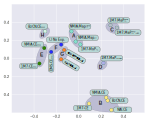
\includegraphics[width=.45\textwidth]{graphs/didy/PCA} \hfill
	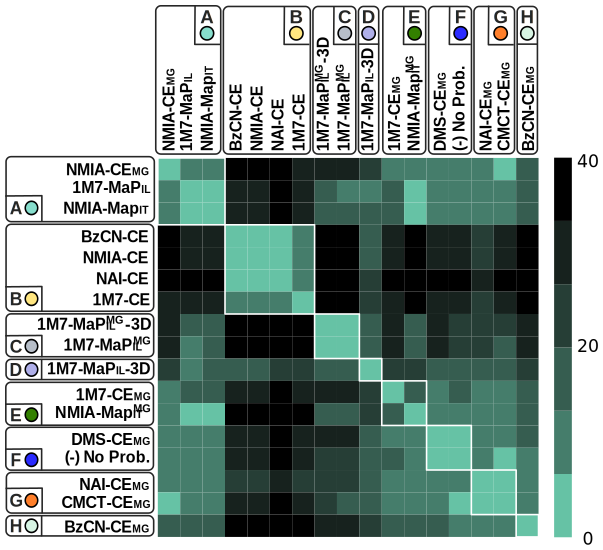
\includegraphics[width=.45\textwidth]{graphs/didy/bi_clustering}\\
	}
		
		This number may not seem to be supported by a inspection Figure 5 (PCA, left above), but it must be reminded that a PCA is simply a projection. Points that are distant in the PCA are typically distant in the original higher-dimensional space, but close points in the PCA may also be quite distant due to the missing depth perception. 
		
		On Figure 5, we already see a clear separation between B, D, C, A, and H. Moreover, merging clusters E, F and G would lead to the aggregation of substantially different conditions, as can be seen in Figure 6 (right above), so we considered 8 conditions.}

	\Comment{The authors compare stop-based to mutation-based experiments. However, the term “stop-based” is somewhat misleading because there is another variable here - the modification assay platform. MaP protocols must be assayed by NGS whereas the stop-based protocols used in this work rely on CE for modification detection. It is possible that the differences observed between MaP and CE data (see e.g., Fig. 5) have little to do with the stop strategy and more with the sequencing platform (CE vs NGS). The use of “stop-based” might create an impression that this feature is necessarily responsible for these differences. The ideal comparison should be between experiments such as SHAPE-MaP and SHAPE-seq, but given that experiments were already performed, I recommend changing the term and clarifying the technical differences between these subsets of conditions.}
	
	\Answer{We agree that SHAPE CE should not be mischaracterized as a representative for all SHAPE protocols based on RT stops (notoriously including SHAPE-Seq). Our descriptions were sometimes misleading in that respect, so we modified and removed the corresponding column in Table 2 and tried to remove any sentence that would involuntarily suggest the superiority of a technology/reagent based on our observations.}

	\Comment{Does IPANEMAP perform better when sampling deeper? More generally, was sample size of 1,000 selected following performance optimization or simply because there is a convention in the field that 1,000 suffices for reproducibility at the base-pair level?}
	
	\Answer{
		We were happy with the overall reproducibility of our results with 1~000 structures, which has been the standard practice in the field since the original \cite{Ding2003} paper. Moreover, our computational requirements scale quadratically with the number of structure, so we recommended a sample size of 1~000, which represents in our opinion a good tradeoff between reproducibility and efficiency.
	
		To address this question more precisely, we reexecuted the \didy benchmark using a sample size of 2~000, and observed a minor non-significant variation in the MCC (\emph{i.e.} the results did not allow to refute the hypothesis of equal expected MCCs for both experiments).}

	\Comment{Table 1 could be moved to the Supp.}
	
	\Answer{We disagree and, while anecdotal, we believe this figure illustrates nicely a case where the addition of data leads to an improvement of the model.}

	\Comment{Table 2 summarizes performance differences at the Mut/Stop and -/+Mg levels. I wonder if such differences could have been detected already at the reactivity level and without the need for Boltzmann sampling. For example, one could lump all “Mut” profiles together as replicates for condition A and all “Stop” profiles as replicates for condition B and then perform differential reactivity analysis to spot differentially reactive regions and their statistical significance.}
	
	\Answer{For this revision, we added a principled comparison of the raw reactivity profiles based on correlation of reactivity. Its results are now included in the supplementary material and reproduced below
	\Quote{\centering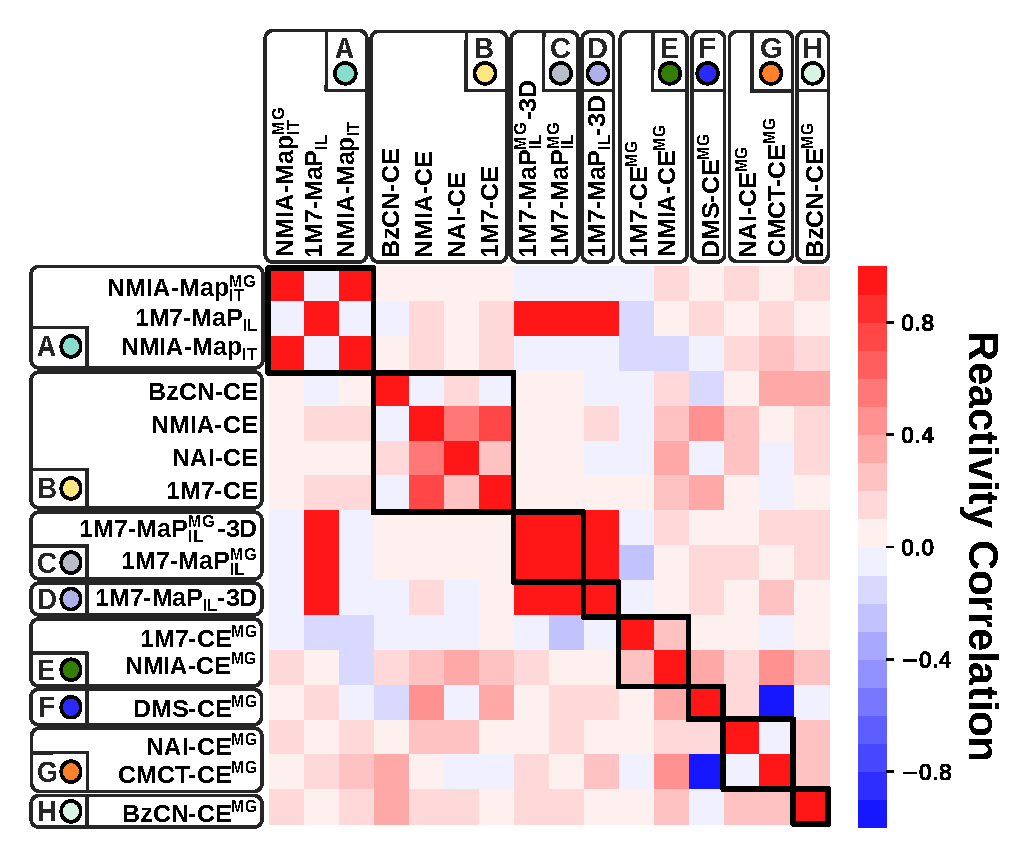
\includegraphics[width=.64\textwidth]{graphs/didy/reactivity_correlation.pdf}}
	As can be seen in this matrix, "MaP" conditions essentially lump in two classes at the reactivity level (that do not fully align with the "MaP" clusters A/C/D). However, "CE" conditions do not form a clear cluster, and in many case correlate better with a "MaP" conditions than with "CE" conditions in the same cluster.
}

	\Comment{In Table 2, the two conditions in cluster C perform quite differently: 74\% and 85\%. Can the authors suggest why this happens? Can the performance differences be picked up by a differential reactivity analysis? For example, there may be a certain differentially reactive region, which the ensemble distance measure does not pick up. }
	
	\Answer{Indeed, the difference can be traced back, for the conditions in C, to a reactivity in the 5' terminal region that is greater for  \OneMSevILUThreeMg than for \OneMSevILUMg, resulting in a loss of the basal helix in the model predicted by \OneMSevILUThreeMg. This variation, coupled with the shift of a small helix, is alone responsible for the change of performances (the MCC does not take prisoners...). }

	\Comment{Does bi-probing improve precision (std) over mono-probing? Similarly, does probing with multiple similar conditions improve precision compared to mono- or bi-probing (Table 3)?}

	\Answer{As stated in the manuscript, bi-probing does not improve the standard deviation of the MCC (8\% for mono-probing, 8.4\% for bi-probing). Considering the sets of similar conditions in Table 3 increases the stdev to around 10\%. However, this observation merely stems from a statistical artifact, as the large number of conditions in Cluster B leads to a multiplication of MCC around 60\%, resulting in what would appear to be a bimodal distribution ($\to$ large variance/stdev) without reflecting any underlying reality.}

	\Comment{Performance assessments in this work focus primarily on averages although precision is an important factor, especially when statistical sampling is involved and large variation in prediction accuracy is observed for different RNAs. The conclusion that one might not gain much or at all from increasing the no. of probes or using similar ones overlooks the notion that redundancy potentially increases our confidence in the results. For example, replicates are inherently redundant and ideally not too diverse, yet they are generated to decrease std around the mean although the mean is always lower than some of the point estimates. A related question is as follows.
	
	For bi-probing, if we repeat predictions with 10 independent Boltzmann samples, which strategy is more precise: averaging predictions between the two probes or the corresponding bi-probing prediction?}

	\Answer{
		The meaning of \emph{averaging the predictions} is unclear to us in this context (our method produces 2D model(s), how does one average models?), and could be interpreted in several ways that we try to cover in the following sentences. 
		
		If the intent is to compare the MCC of a bi-probing prediction with the average of the two mono predictions, this is precisely the content of Figure 7.B, and our analysis does not reveal a substantial reduction of the stdev.
		
		The intent may also be to compare, for a given pair of conditions, the stdev of the MCC to the stdev of the mean MCC over two independent mono executions (by running several experiments). In this setting, we either analyze a single pair, and obtain results that are probably not significant, or we need to report summary statistics over stdevs of a dataset of pairs of conditions, something that would not only be heavily time-consuming, but also hard to interpret. We will welcome clarification over this point over the next round of reviews.
		
		However, if the objective metric of quality is the reproducibility of predictions using \OurTool (\emph{i.e.} to decrease the stdev as low as possible), a very simple solution is to perform 10+ independent runs of \OurTool, and elect the dominant conformation. Indeed, in most cases, \OurTool produces a well-defined structure with high probability, as suggested by Figure 8 (WT) and 9. By running \OurTool repeatedly, the frequency of the dominant structure becomes an estimator, with variance decreasing on the number of iterations, for the emission probability of the structure. This process ultimately converges towards a deterministic election of the most probable structure, and should already be fairly close to determinism after 10 iterations. Moreover, the time requirement scales linearly with the number of iterations, as opposed to quadratically if one were to multiply the number of samples. 
		
		In the future, we also wish to report, and letting the user specify, a \Def{random seed}, which will  allow the exact reproduction of an analysis. 
		However, such a feature is currently not supported by \Software{RNAsubopt}, so we must first work towards its inclusion to the \Software{ViennaRNA} package.
		}


	\Comment{Table 5: I do not think it demonstrates a significant finding. All subsets include $1M7-MaP_{IL}^{MG}$, whose mono performance is already 0.85, as compared to 0.853. According to Table 2, it is the best-performing condition. My guess is that the 0.003 gain is an artifact rather than a manifestation of complementary information embedded in the additional conditions. If the point made is that it’s advantageous to jointly analyze conditions rather than average them out, then I think it could be made in the context of the other results. However, as shown here, using too many conditions might negatively affect performance, so not sure if robust guidelines can be derived from these results.}
	
	\Answer{Upon further inspection of the prediction, it appears that the reviewer's intuition is correct and the improvement in comparison to the best of the group is marginal. We have removed the Table, and any mention to those specific triplets in the text.}

	\Comment{Fig. 9: $1M7-MaP_{IL}^{MG}$ is a top performer on the Lariat data per Table 2, but its MCC variance over 10 runs is high per Fig. 9. If I interpret Fig. 9 correctly, the 85\% MCC from Table 2 is not shown for this condition and maybe resulted from another IPANEMAP run. In any case, I wonder if Table 2 lists the results of single runs or averages over 10 runs. If single runs are listed, how representative are they for the two conditions with high variances (Fig. 9)? Maybe replace them with average runs? Same questions for results with multiple probes. Note that the case for $NMIA-MaP_{IT}$ is similar as 80\% seems to be max performance.}
	
	\Answer{
		We would like to sincerely thank this reviewer for noticing and voicing this apparent inconsistency, which led us to realize a severe mistake in Figure 9. For reasons to be determined, the labeling of the y-axis (MCC) ended up being dilated, showing MCCs in the 70\%/82\% range. The revised version of Figure 9, reproduced below, now features corrected axis and is now consistent with the averages MCC reported in Table 2.
		\Quote{
				{\centering
					\begin{minipage}{.58\linewidth}
					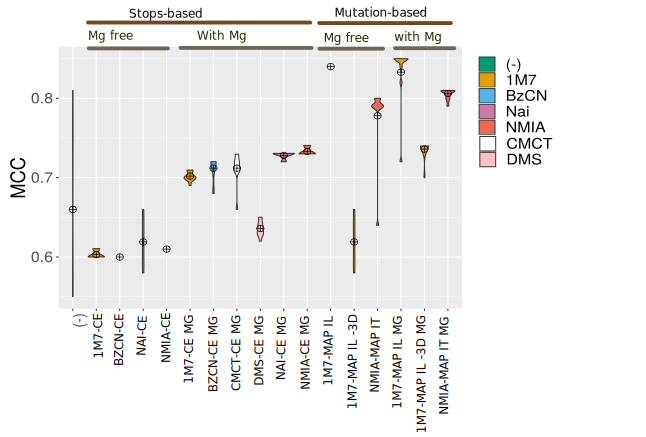
\includegraphics[width=\linewidth]{graphs/boxplotreproducibility}
					\end{minipage}\hfill
					\begin{minipage}{.4\linewidth}
	\Heatset{min=60,   
		max=83,   
		max colour=Aquamarine3, % colour at maximum
		min colour=BadCol,      % colour at minimum
		Min colour=BadCol, % colour for values below min
		Max colour=Aquamarine3   % colour for values above max
	}
					\newcommand{\M}[1]{\multicolumn{1}{l}{#1}}
						\begin{adjustbox}{max width=\linewidth}
							\begin{tabular}{@{}lccHHH}
								\toprule
								&          &           & \multicolumn{3}{@{}c@{}}{MCC\%}              \\
								Condition                   &  Clust.  & Mg$^{2+}$ & \M{\relsize{-1}\OurTool} & \M{MFE} & \M{MEA} \\ \midrule
								\OneMSevILUMg               & \Bull{C} &    \Mg    & 85                       & 82      & 82      \\
								\OneMSevILU                 & \Bull{A} &   \NoMg   & 84                       & 82      & 84      \\
								\NMIAMg                     & \Bull{A} &    \Mg    & 81                       & 80      & 80      \\
								\NMIA                       & \Bull{A} &   \NoMg   & 80                       & 69      & 69      \\
								\OneMSevILUThreeMg          & \Bull{C} &    \Mg    & 74                       & 75      & 75      \\
								\NMIAMgCE                   & \Bull{E} &    \Mg    & 73                       & 72      & 73      \\
								\NAIMg                      & \Bull{G} &    \Mg    & 73                       & 68      & 70      \\
								\BzCNMg                     & \Bull{H} &    \Mg    & 71                       & 68      & 54      \\
								\OneMSevMgCE                & \Bull{E} &    \Mg    & 70                       & 69      & 70      \\
								\CMCTMg                     & \Bull{G} &    \Mg    & 70                       & 68      & 73      \\
								\OneMSevILUThree            & \Bull{D} &   \NoMg   & 64                       & 56      & 61      \\
								\DMSMg                      & \Bull{F} &    \Mg    & 63                       & 66      & 67      \\
								\NMIACE                     & \Bull{B} &   \NoMg   & 61                       & 60      & 60      \\
								\OneMSevCE                  & \Bull{B} &   \NoMg   & 60                       & 61      & 61      \\
								\BzCN                       & \Bull{B} &   \NoMg   & 60                       & 59      & 59      \\
								\NAICE                      & \Bull{B} &   \NoMg   & 60                       & 59      & 59      \\ \midrule
								Avg Technology              &          &  $-$  & 78                       & 74      & 75      \\
								&          &  $-$  & 66                       & 65      & 65      \\
								Avg -/+ Mg$^{2+}$           &          &   \NoMg   & 67                       & 64      & 65      \\
								&          &    \Mg    & 73                       & 72      & 71.5    \\ \midrule
								{\bfseries Average overall} &          &  $-$  & 70.5                     & 68      & 68.5    \\ \bottomrule
								&          &           &                          &
							\end{tabular}
					\end{adjustbox}
					\end{minipage}
					\\}
		}
		
		Average MCC values over 10 runs are indeed reported in Table 2, and an independent dataset was generated to create Figure 9, leading to minor discrepancies. For multiple probes, only a single result was generated.
	}

	\Comment{Page 8, line 55: 1000 samples or 1000 structures per condition?}
	
	\Answer{Fixed.}

	\Comment{Methods, page 3: The definition of highly similar clusters uses a default value $\delta=1$. My understanding is that this means that highly similar clusters must have the exact same centroids, such that minor variation is not allowed. Is that correct?}
	
	\Answer{Two centroids distant by at most one base-pair (included) will be deemed highly similar, so a (very) minor variation will be tolerated.}

	\Comment{Methods, page 3: Is $E_{d}(S)$ the pseudo-energy term of the total score or is it the entire score, including the NNTM free-energy? }
	
	\Answer{$E_{d}(S)$ denotes the entire score, including NNTM free energy plus the energy bonus.}

	\Comment{My impression is that the main purpose of the clustering was to detect the outliers in cluster B. Since I find this to be a technical piece of the entire analysis, and not a very interesting one, I suggest moving most of the text + Fig. 5 \& 6 to the Supp.}
	
	\Answer{We already addressed this comment above, and respectfully disagree with this assessment.}

	\Comment{Page 5, benchmarks on Cordero et al.’s dataset: It is noted that the prediction is the centroid of the largest probability cluster. My understanding, based on the method’s section, is that the prediction should be the centroid of the pareto-optimal clusters. It is unclear whether this is a modification of the method, and if yes, if it applies to all other benchmarks or not. Please clarify. }
	
	\Answer{In a mono-probing setting, due to properties of the two criteria used for the multi-objective Pareto optimization, it is rigorously impossible for \OurTool{} to return more than one cluster.  Indeed, the cluster $C^\star$ having max stability $s^\star$ is such that: either $C$ has support $t^\star=1$, in which case it dominates any other cluster with signature $(s<s^\star,t\in\{0,1\})$; or $C$ has support $t^\star=0$, ruling out the possibility of $t=1$ for any other cluster (since it would imply $s>s^\star$). Note that \OurTool also reports dominated clusters for furter inspection.
	}

	\Comment{Page 10, line 56: Figure 3 should be Table 3.\label{comment:last}}

	\Answer{Fixed.}
	
	
\end{enumerate}

\bibliographystyle{abbrvnat}
\bibliography{biblio}
\end{document}
